\chapter{CDRF: A Large-Scale RF Benchmark and Toolkit for Drone Detection, Classification, and Open-Set Recognition}
\label{chap:cdrf}

\section{Introduction}
\label{sec:introduction}

% \textbf{Framework Context:} 
The development of wireless foundation models requires validating a fundamental hypothesis: can representations learned by vision models transfer effectively to the wireless domain? Chapter~\ref{chap:denomae} proposes that multimodal masked autoencoders can learn universal wireless signal representations by treating signals as images (spectrograms, constellation diagrams). Before pursuing this costly self-supervised learning approach, we must first establish that vision architectures (YOLO for detection, ResNet for classification) can indeed extract meaningful features from RF signals represented as spectrograms. This chapter addresses Research Question 1 (RQ1) through a practical validation: the CageDroneRF (CDRF) benchmark demonstrates that pre-trained computer vision models successfully transfer to wireless perception tasks, providing empirical evidence for the cross-modal transfer principle underlying our modular framework.

Beyond this theoretical validation, CDRF serves a critical practical role: providing a realistic, stress-tested benchmark for evaluating foundation model components. While many wireless datasets capture signals under idealized laboratory conditions, operational deployment demands robustness to low signal-to-noise ratios (SNR), spectrum interference, frequency offsets, and domain shifts (indoor$\leftrightarrow$outdoor). CDRF's raw-signal augmentation pipeline and diverse collection methodology create exactly these challenging conditions, enabling us to assess whether foundation model approaches generalize beyond clean benchmarks to real-world scenarios.

The rapid proliferation of Unmanned Aerial Vehicles (UAVs) provides a compelling application domain for this validation. UAVs enable transformative applications in logistics, agriculture, and emergency response~\cite{robotics12020053}, while introducing risks to safety, privacy, and critical infrastructure~\cite{nguyen2025effective}. Traditional sensing modalities (radar, vision, acoustics) exhibit notable limitations: environmental sensitivity, limited small-target range, line-of-sight dependence, and high deployment costs. Radio-Frequency (RF) sensing offers complementary advantages: continuous command-and-control links enable day/night, non-line-of-sight detection at low cost, with RF captures carrying rich device, protocol, and operator signatures~\cite{mo2022deep}.

Despite these advantages, progress in Machine Learning (ML) for RF-based drone perception has lagged behind vision and language domains, precisely the gap motivating this dissertation's framework. A central barrier is the absence of broad, standardized benchmarks that test models under realistic stress conditions. Existing datasets are often narrow in class diversity, limited in volume, collected in clean environments with restricted SNR ranges and weak interference diversity. Models trained on such data overfit to idealized conditions, achieving near-perfect scores on ``easy'' benchmarks yet degrading severely in operational deployments with Bluetooth/Wi‑Fi interference, spectrum crowding, and low SNR, exactly the conditions that foundation models must handle~\cite{rfuav}.

We introduce CageDroneRF (CDRF), a benchmark built to close this gap with a dataset-and-toolkit co-design. CDRF comprises real-world captures from controlled RF-cage facilities and open-campus settings, paired with a principled raw‑signal augmentation pipeline that programmatically varies SNR, injects interfering emitters, and applies frequency shifts while preserving label consistency. Crucially, augmentations operate on complex baseband I/Q, before time-frequency conversion, so synthesized conditions faithfully reflect RF phenomena rather than image-level artifacts. For detection, frequency shifts are accompanied by exact recalculation of You-Only-Look-Once (YOLO~\cite{redmon2016you})-format annotations with correct wrap-around behavior on the spectrogram’s frequency axis. The data processing stack converts raw captures to spectrograms via Short-Time Fourier Transform (STFT) and exposes all parameters (e.g., sampling rate, FFT size, segment length) for reproducible ablations and reprocessing.

Beyond the dataset, CDRF provides interoperable utilities for dataset creation, cleaning, and evaluation. The data module loads .dat files via memory mapping, slices long recordings into time windows, generates spectrograms, appends per-sample metadata (including time bounds), and optionally adds controlled AWGN, Rician, or Rayleigh fading noise for precise SNR targets. The YOLO toolkit includes raw‑IQ augmentation and automatic bounding‑box recomputation; a dataset cleaner aligns third‑party releases (e.g., Roboflow-style~\cite{roboflow_website}) into a consistent hierarchy; and a lightweight patch exposes per-detection class probabilities from YOLO for richer calibration and analysis. For classification, CDRF ships PyTorch~\cite{paszke2019pytorch} baselines (binary and multi‑class) built on ResNet‑18~\cite{he2016deep} with ready-to-run dataloaders for both spectrogram images and array/pickle formats, standardizing training, metrics, and confusion matrices. All tooling is dataset-agnostic, enabling applications to use existing public datasets to facilitate cross-benchmark comparability.

Collectively, CDRF aims to shift the field from narrow, clean benchmarks toward realistic, stress-tested evaluation under varied SNRs, interference, and frequency offsets, conditions that operational systems routinely encounter. By releasing both data and the underlying signal-first augmentation/evaluation stack, we seek to catalyze reproducible research on RF-based detection, identification, and related perception tasks. We summarize our key contributions as follows:
\begin{itemize}
    \item \textbf{CDRF benchmark dataset:} Real-world RF captures from cage environments with standardized spectrogram generation and rich per-sample metadata.
    \item \textbf{Raw‑signal augmentation pipeline:} Controlled SNR injection, interfering-signal mixing, and frequency shifts applied at I/Q level, with exact YOLO label recomputation (including wrap-around).
    \item \textbf{SNR-structured datasets:} Programmatic creation of SNR‑stratified splits (including noise-only backgrounds) for stress testing and realistic robustness evaluation.
    \item \textbf{Interoperable tooling:} Open-source utilities for dataset creation, metadata generation, Roboflow-style cleaning, and spectrogram rendering; tools are dataset‑agnostic for use on existing releases.
    \item \textbf{Detection analysis enhancements:} Patch exposing per-detection class probabilities from YOLO to support calibration studies and open-set analyses.
    \item \textbf{Baselines and evaluation:} Ready-to-run PyTorch baselines for binary and multi-class classification with standardized metrics and confusion matrices, enabling reproducible benchmarking across tasks.
    \item \textbf{Open set recognition:} Implementation of open-set recognition capabilities to handle previously unseen classes during inference.
    % \item \textbf{Multi-label classification:} Support for multi-label classification tasks, allowing models to predict multiple classes simultaneously.
    % \item \todo{open-set and multi-class?}
\end{itemize}

Within the broader dissertation framework, CDRF serves as a critical validation domain demonstrating cross-modal knowledge transfer. By converting RF signals to spectrogram images, this work validates that vision models (YOLO, ResNet) can transfer learned representations to wireless perception tasks, a key principle underlying the multimodal approach in DenoMAE (Chapter~\ref{chap:denomae}). This empirical validation provides the foundation for the dissertation's modular, cost-effective approach: rather than training wireless foundation models from scratch, we can strategically leverage pre-trained vision architectures (proven here), integrate LLM reasoning (Chapter~\ref{chap:plugandplay}), and enable rapid adaptation via meta-learning (Chapter~\ref{chap:meta_task}). CDRF provides the realistic, stress-tested benchmark needed to evaluate whether these foundation model components generalize beyond clean laboratory conditions to operational deployment scenarios.

The remainder of this paper is organized as follows. Section~\ref{sec:related_work} reviews related work in RF-based drone detection, covering various sensing modalities and existing public datasets. Section~\ref{sec:dataset} details the design and collection of the CDRF dataset, and Section~\ref{sec:data_processing} describes our data preprocessing, augmentation, and annotation pipeline. Section~\ref{sec:ml_tasks} presents the experimental setup and benchmark results for several machine learning tasks, including drone detection, single-label, open-set, and hierarchical classification. Finally, Section~\ref{sec:crdf_conclusion} concludes the paper and discusses future research directions.

\section{Related Work}
\label{sec:related_work}

This section briefly positions CDRF within the existing landscape and highlights the specific gaps it addresses.

Despite growing public datasets, persistent challenges remain: lack of diversity in device classes and environments, restricted raw I/Q access, poorly characterized SNR distributions, scarcity of real-world negative samples, and absence of integrated augmentation and evaluation frameworks. Existing datasets often achieve high in-benchmark accuracy but exhibit poor real-world generalization due to clean collection conditions~\cite{elyousseph2024robustness, gluge2024robust}.

CDRF addresses these gaps by providing: (1) real-world cage and outdoor captures with controlled SNR stratification, (2) raw-signal augmentation pipeline operating at I/Q level with exact label recomputation, (3) dataset-agnostic tooling for spectrogram generation and evaluation, and (4) enhanced detection analysis exposing per-class probabilities for calibration and open-set studies.



\section{CDRF: Design and Collection}
\label{sec:dataset}

In the CDRF dataset, we aim to cover the RF signals emitted from the most common UAV-related devices in the market, including the downlink video signals and uplink Remote Controller (RC) signals. We start building the dataset by recording the UAV signals in a rather clean RF environment, in order to emphasize the characteristics of the signals of interest, and also relieve the impact of interfering RF sources or environmental variations. The clean data can also help on reducing the efforts on data-preprocessing and any following data augmentation processes. 

\subsection{Data Acquisition Platform}
We built the data collection platform using a Software-Defined Radio (SDR) based system. In order to create an RF-isolation platform, we built a customized Faraday cage and placed both the SDR card and receiving antenna inside the cage to mitigate the interfering RF signals. The hardware setups and platform configurations are shown in Fig.~\ref{fig:equipments}. 

We use a Lenovo IdeaPad Flex 5 as the data sink. The machine is equipped with an 8-core Intel Core i7-1165G7 CPU and 16 GB of memory. The operating system running on the machine is Ubuntu 24.04.2 LTS. The data collection flow and scripts are built through GNU Radio v3.10 to bridge the Universal Software Radio Peripheral (USRP) B200-mini for RF signal receiving and processing. The SDR device is then connected to a dual-band omnidirectional antenna, which is attached to a customized mount unit to ensure the antenna is static during data collection. 

To ensure comprehensive coverage of drone transmissions, we employ sweep scanning across relevant frequency bands during data collection. This approach allows us to detect and record signals from devices operating at variable frequencies.
    
\begin{figure}[!t]
    \centering
    \begin{subfigure}[h]{0.45\columnwidth}
        \centering
        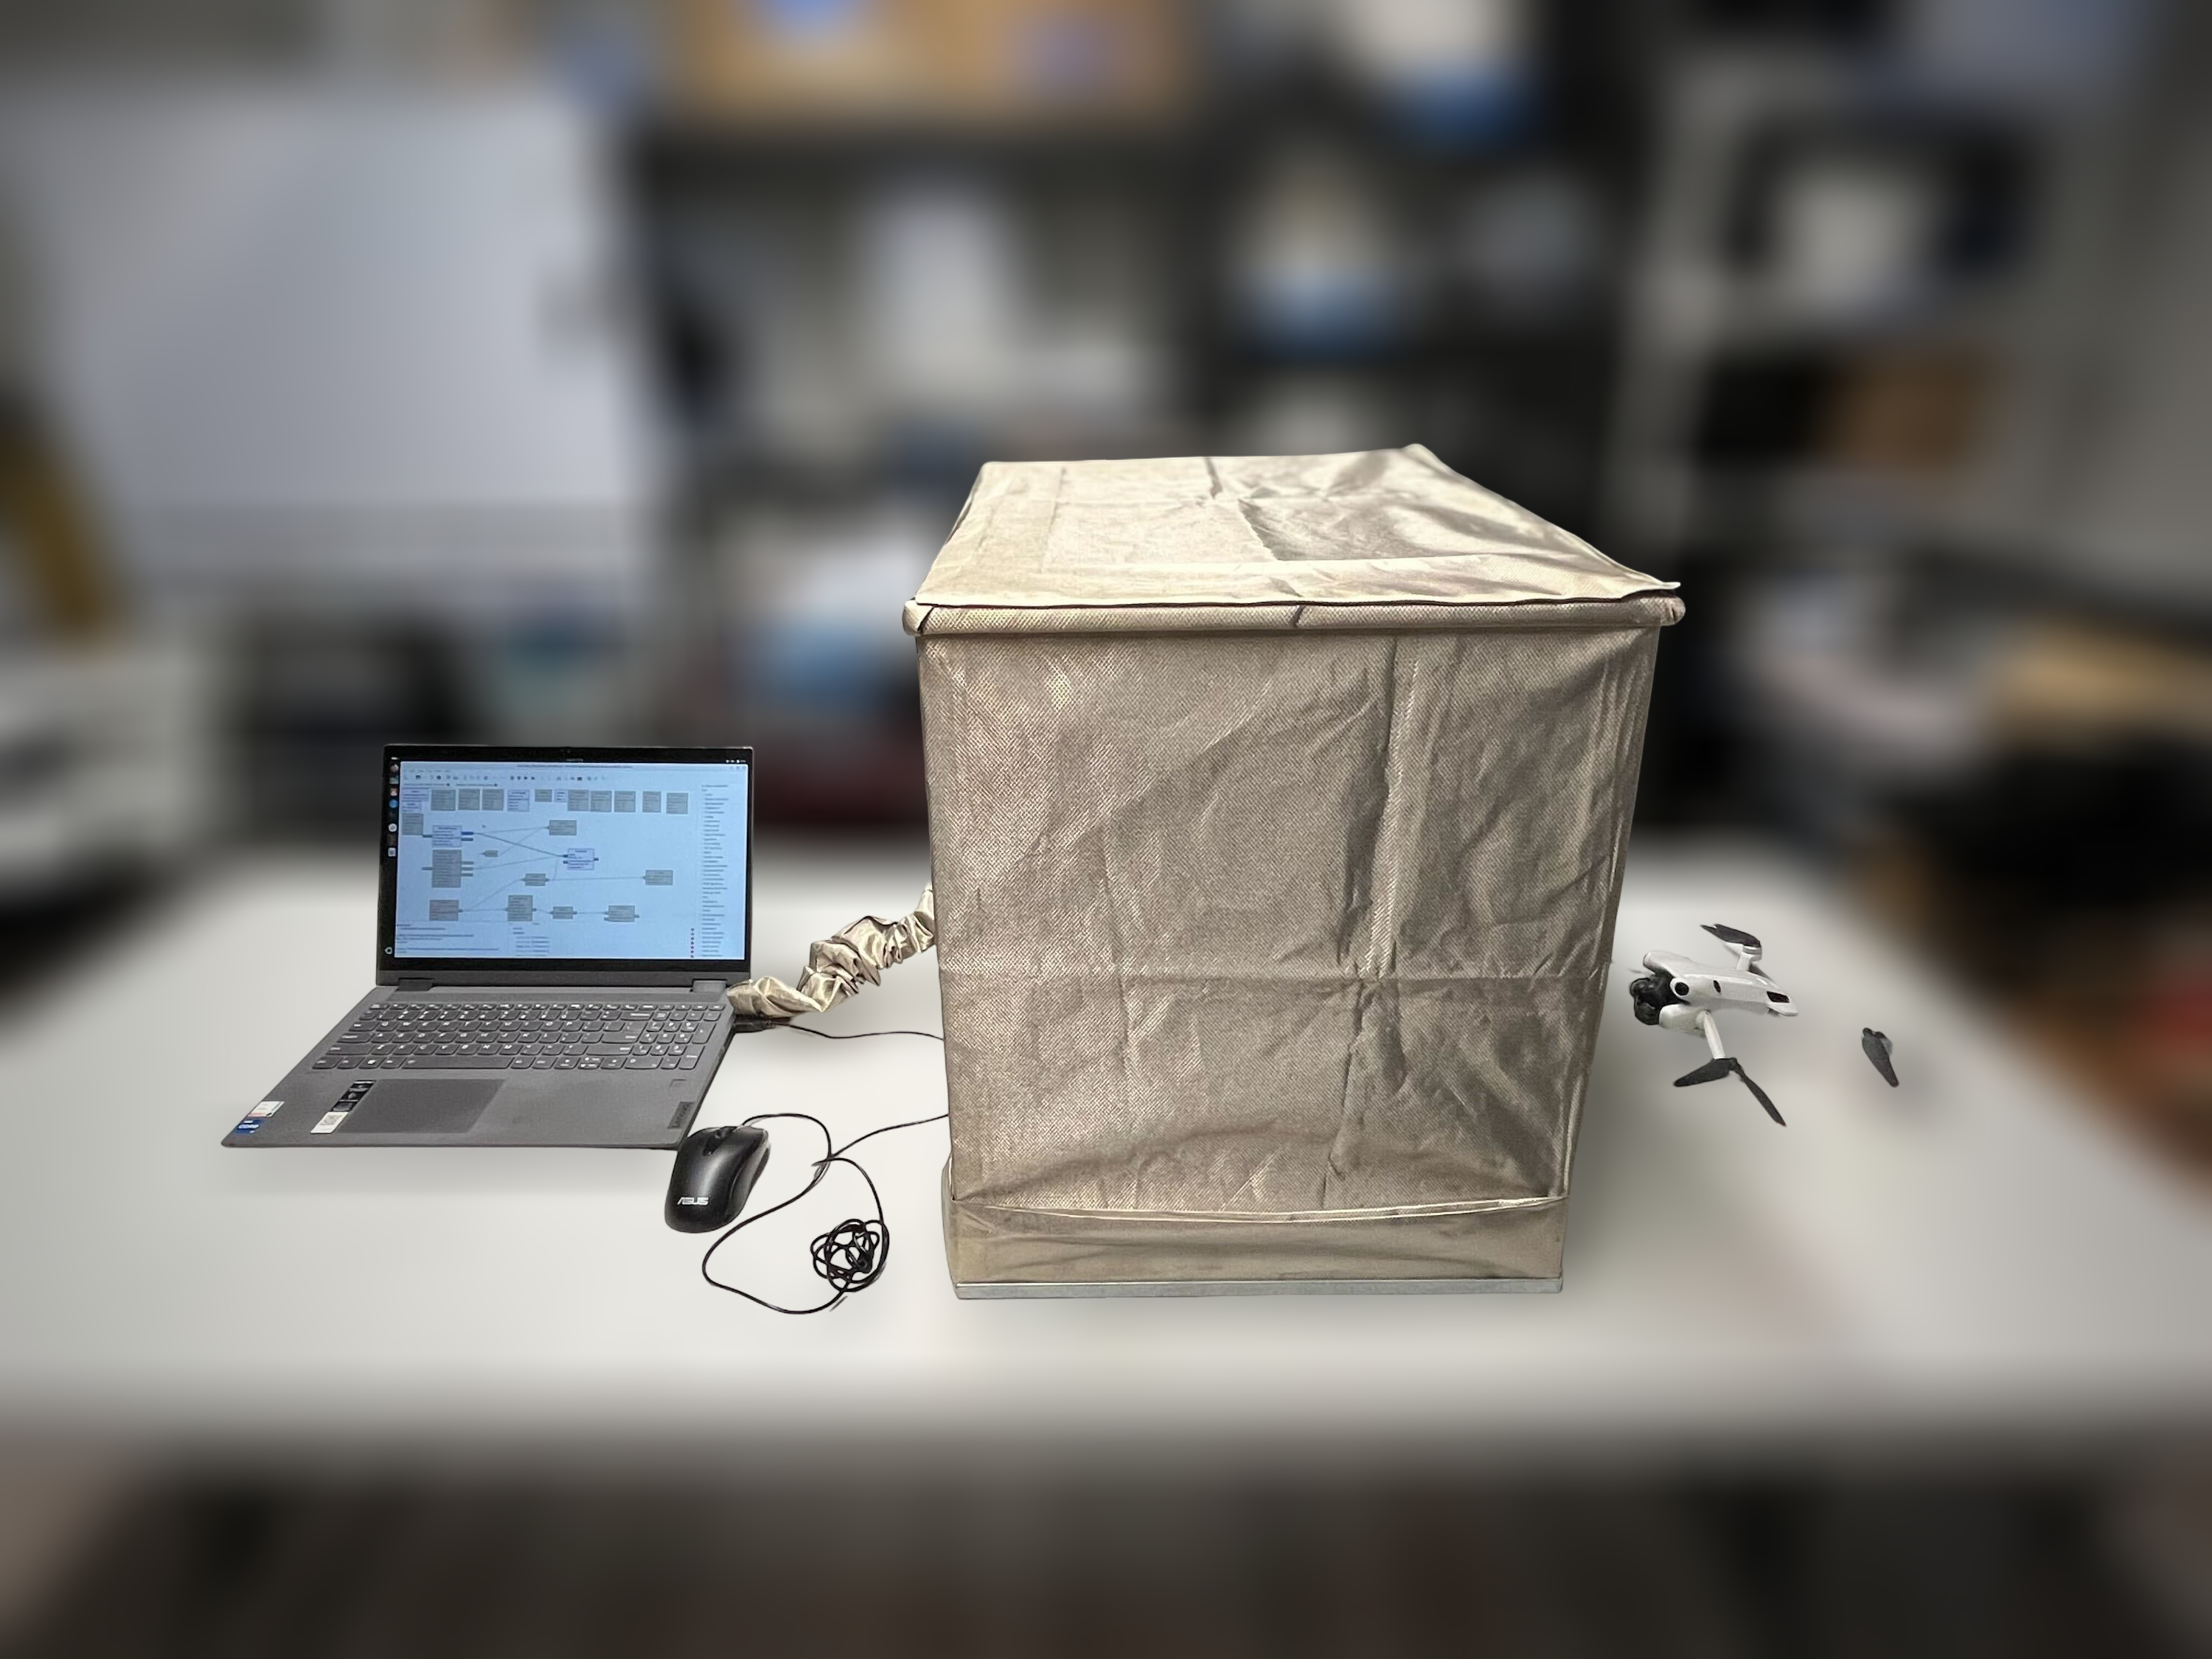
\includegraphics[width=\columnwidth]{FIGURES/cdrf/equipment_cage_closed.jpg}
        \caption{Recording configuration.}
    \end{subfigure}
    \hfill
    \begin{subfigure}[h]{0.45\columnwidth}
        \centering
        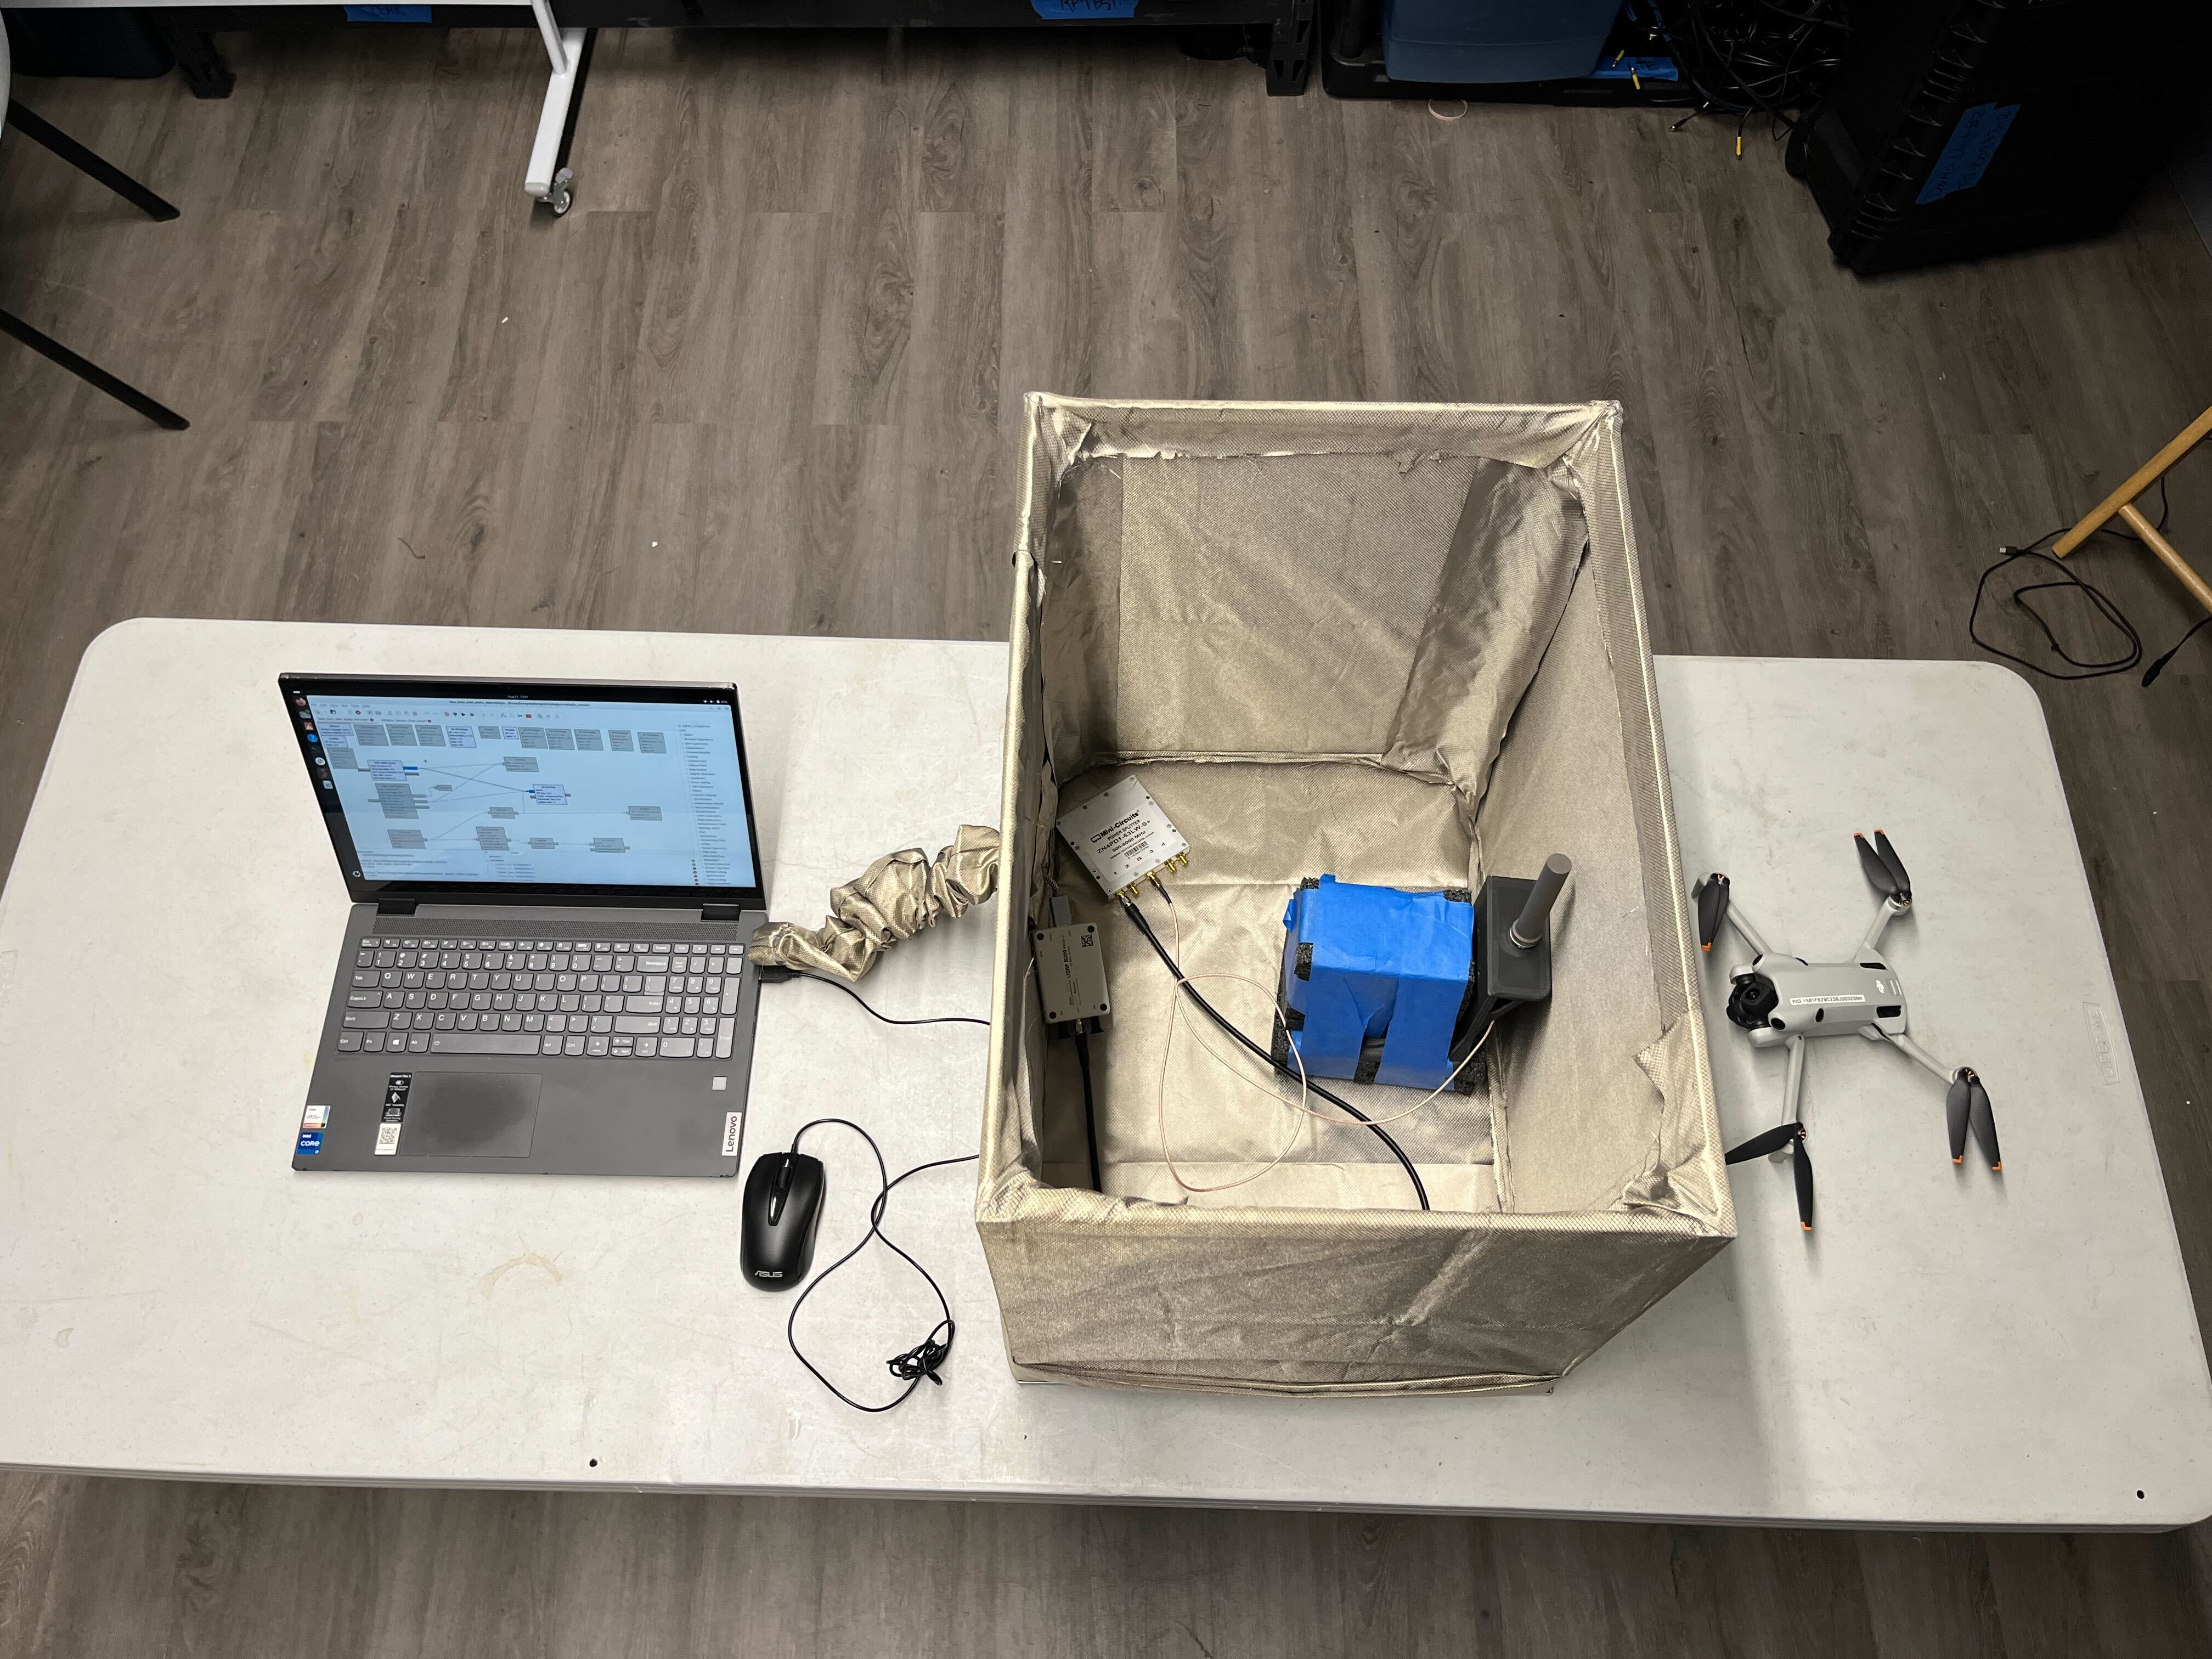
\includegraphics[width=\columnwidth]{FIGURES/cdrf/equipment_cage_open.jpg}
        \caption{Recording equipments.}
    \end{subfigure}
    \caption{Equipment used to capture the data: portable RF shielded enclosure, SDR Card, a laptop, and a drone.}
    \label{fig:equipments}
\end{figure}

\subsection{Data Collection Methodology}
To initiate the data collection, we set up the platform as described in Fig. \ref{fig:equipments} (a), then turn on the UAV and the binding controller. While leaving the antenna inside the cage, we place the UAV outside and at a very close distance to the antenna. This placement ensures that the UAV signals delivered to the antenna are strong enough, while other inferencing RF sources in the surrounding areas are at further distances, and thus their signals will be mostly blocked by the Faraday cage. In addition, the RC of the UAV is kept in another room next to the one where the data is collected. Our goal is to minimize the RC signals captured by the collection platform in this phase, so that the dataset can support further analysis on UAV signals and RC signals separately. This can also provide more flexibility for further data augmentation. 

\begin{figure}[!t]
    \centering
    \begin{subfigure}[h]{0.45\columnwidth}
        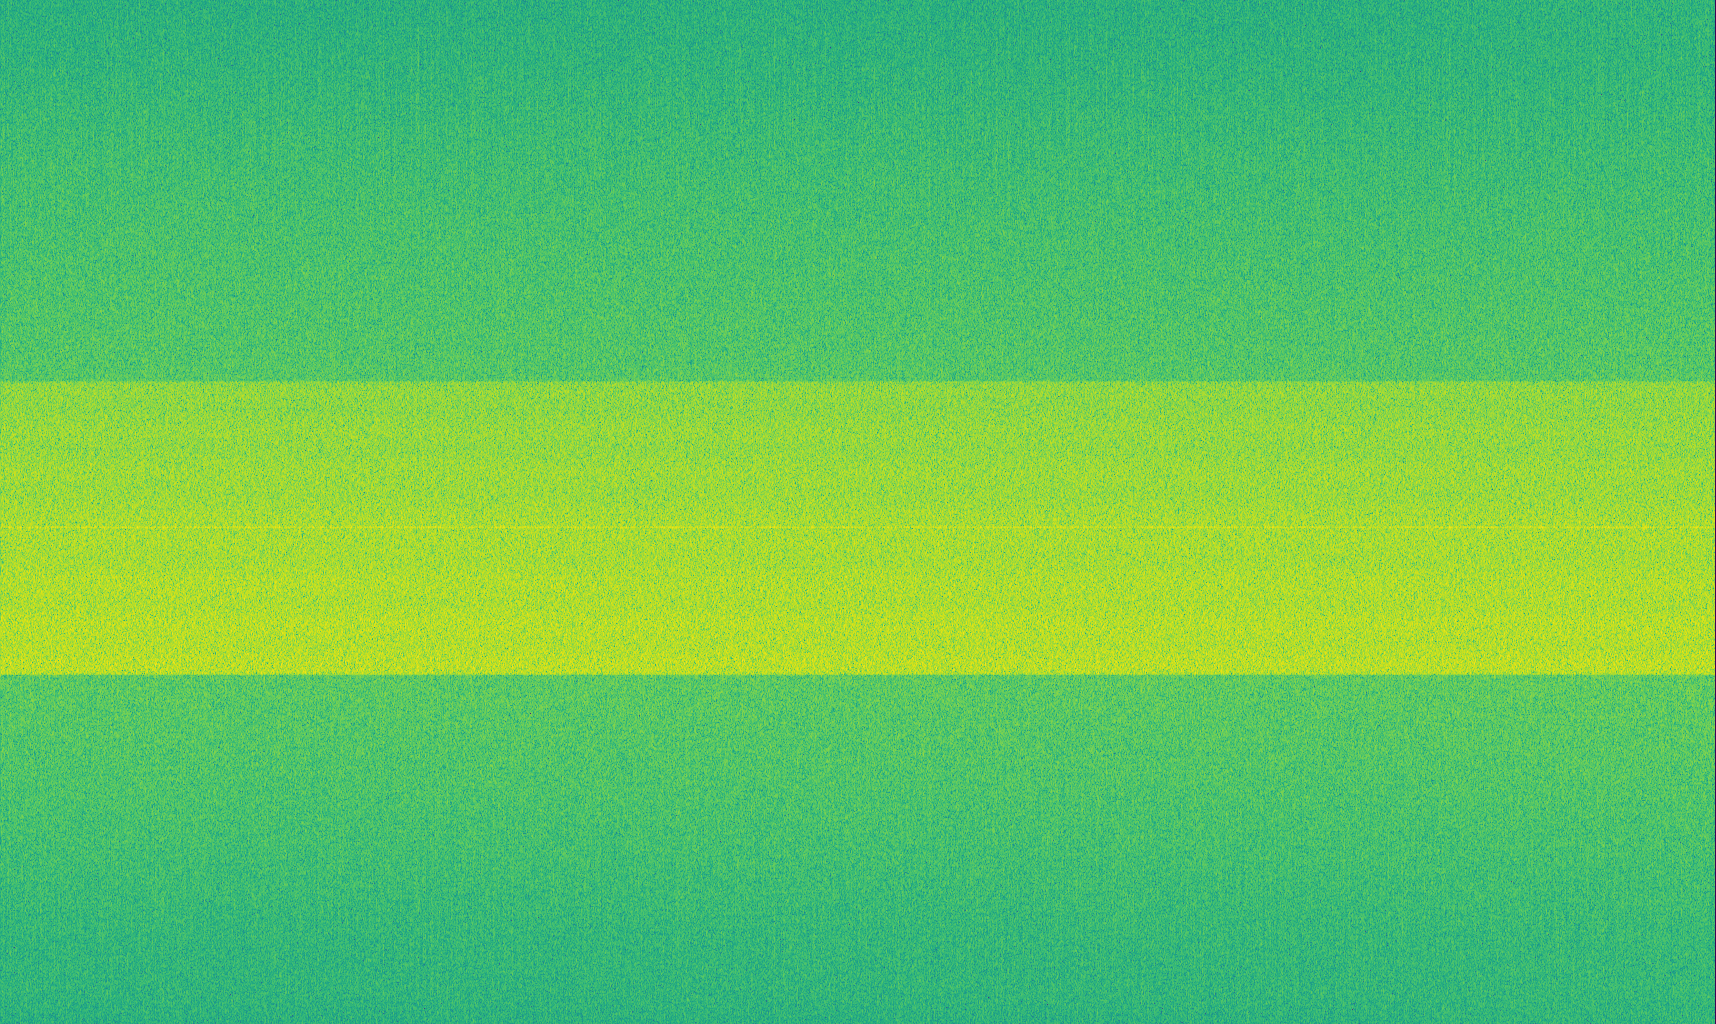
\includegraphics[width=\columnwidth]{FIGURES/cdrf/Autel_Xstar_5_918_sample_106.png}
        \caption{Autel X-Star}
    \end{subfigure}
    \begin{subfigure}[h]{0.45\columnwidth}
        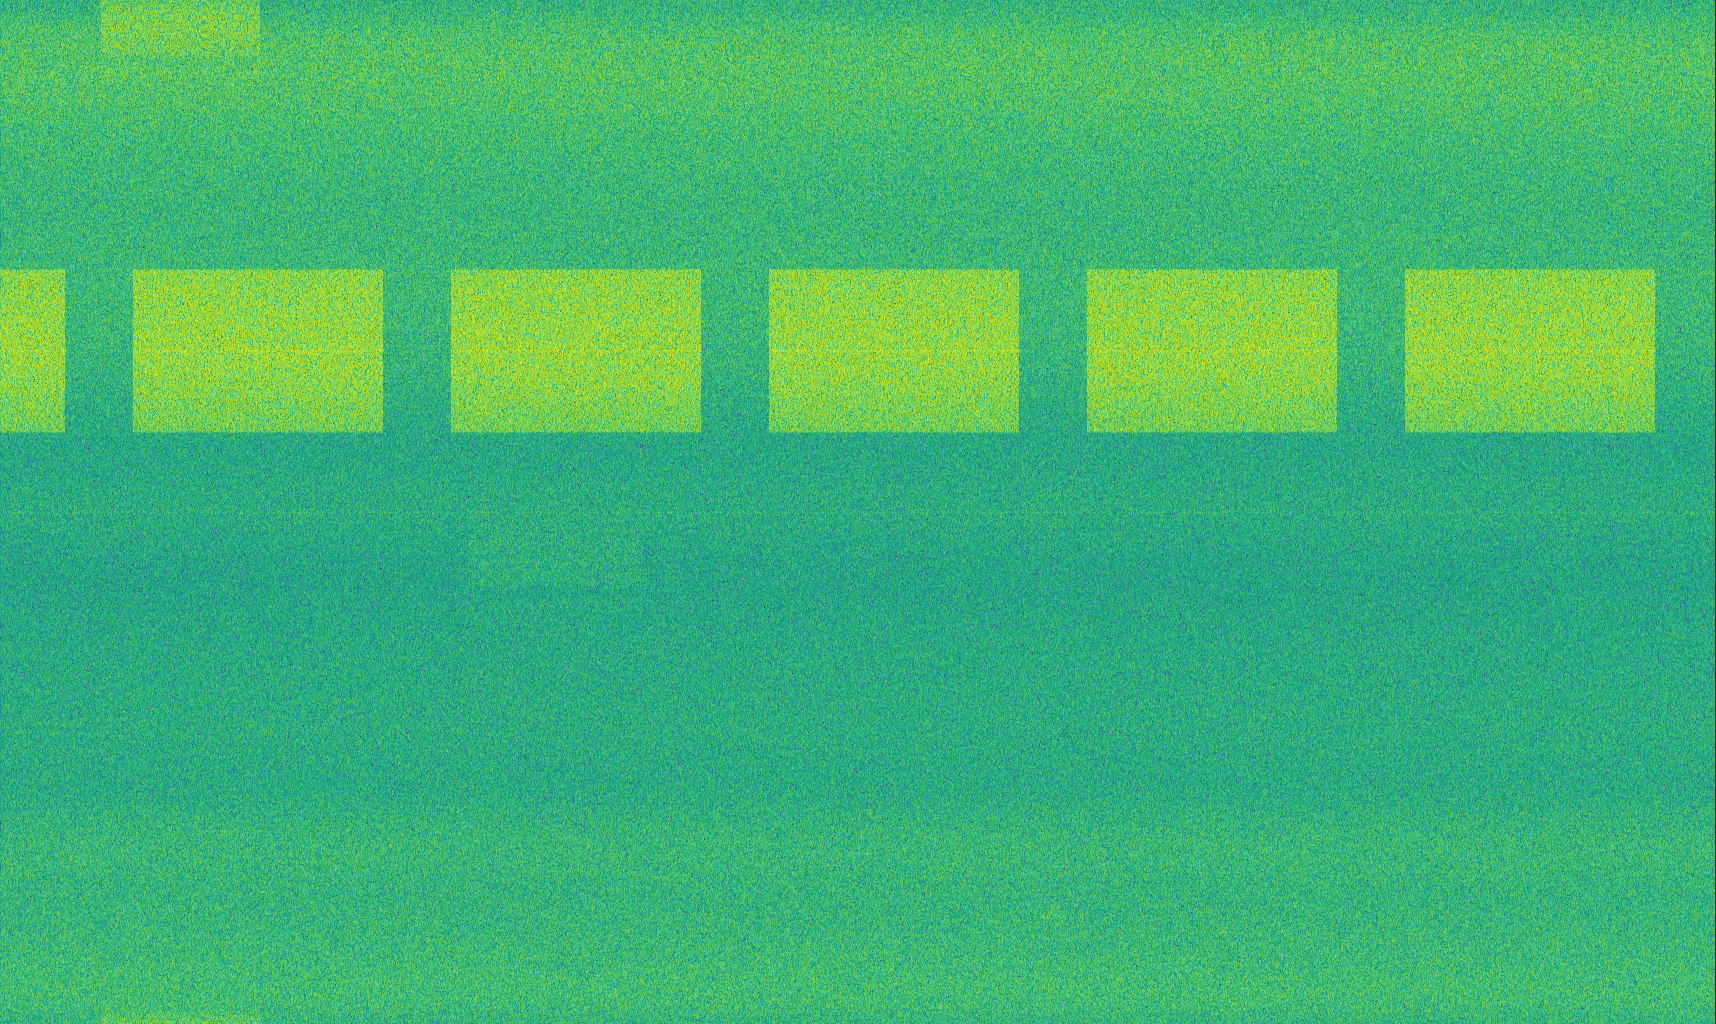
\includegraphics[width=\columnwidth]{FIGURES/cdrf/Autel_EXOII_10_2457_vis_sample_282.png}
        \caption{Autel EXOII}
    \end{subfigure}
    \begin{subfigure}[h]{0.45\columnwidth}
        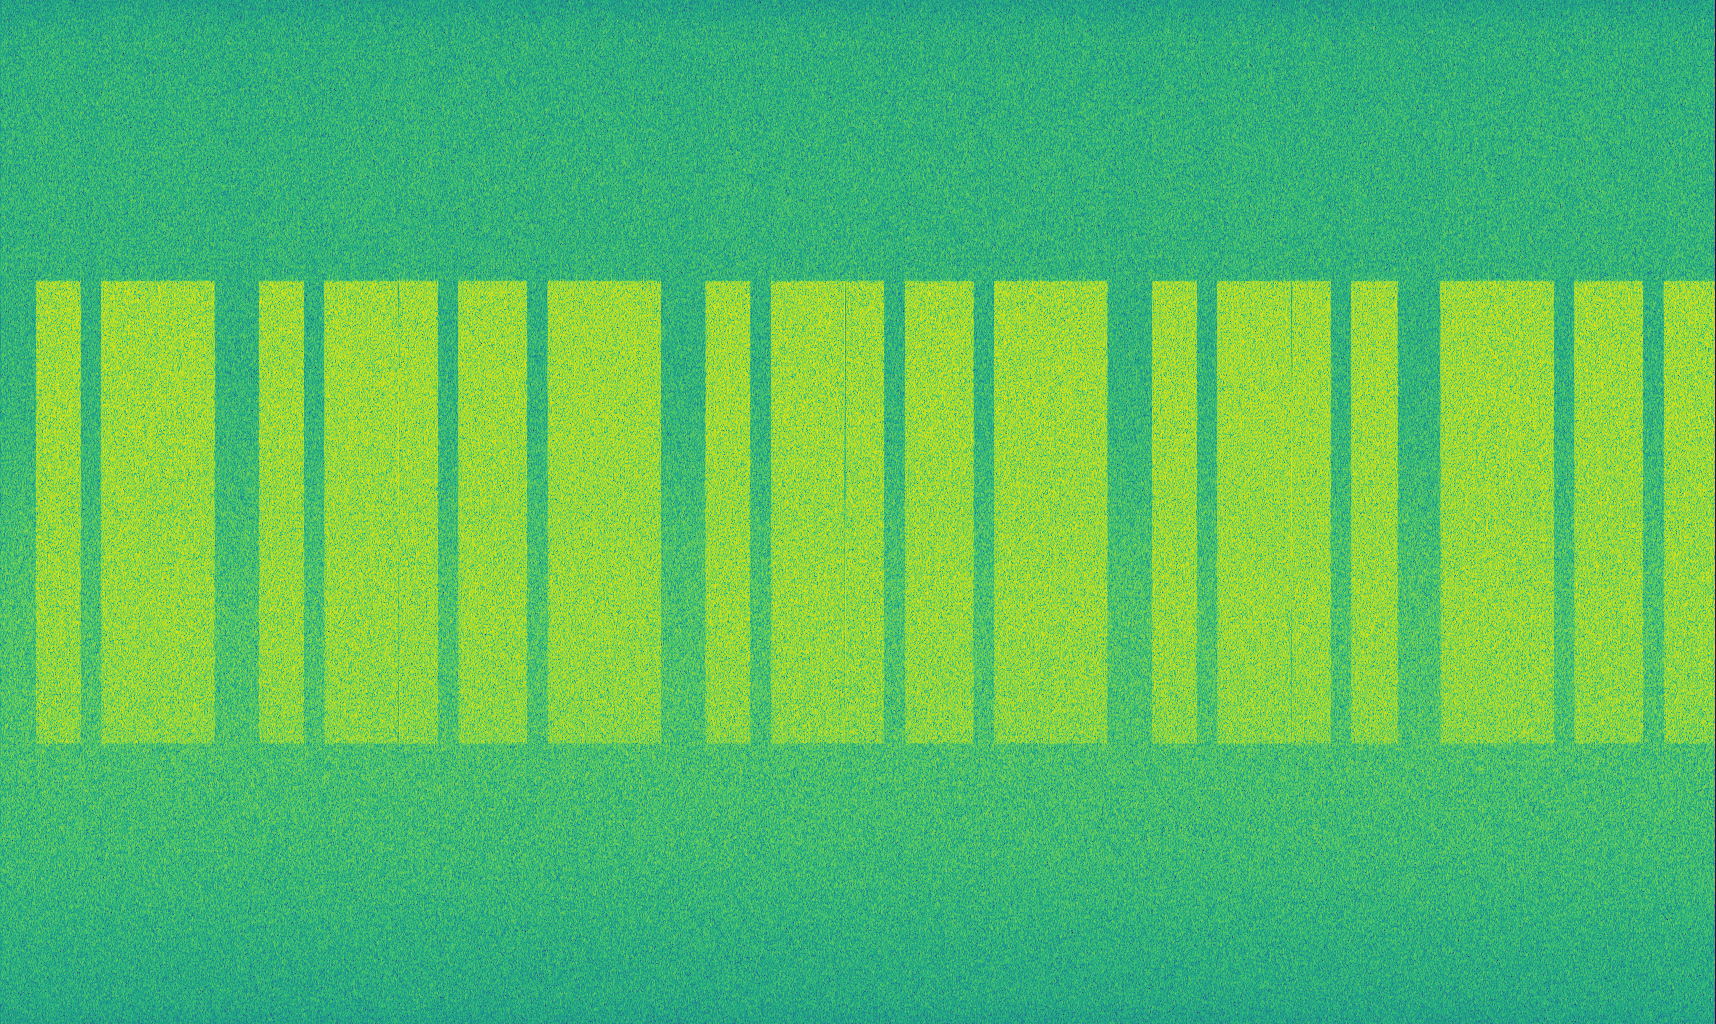
\includegraphics[width=\columnwidth]{FIGURES/cdrf/DJI_Mavic2Pro_10_2442_not_engaging_sample_9.png}
        \caption{DJI Mavic 2 Pro}
    \end{subfigure}
    \begin{subfigure}[h]{0.45\columnwidth}
        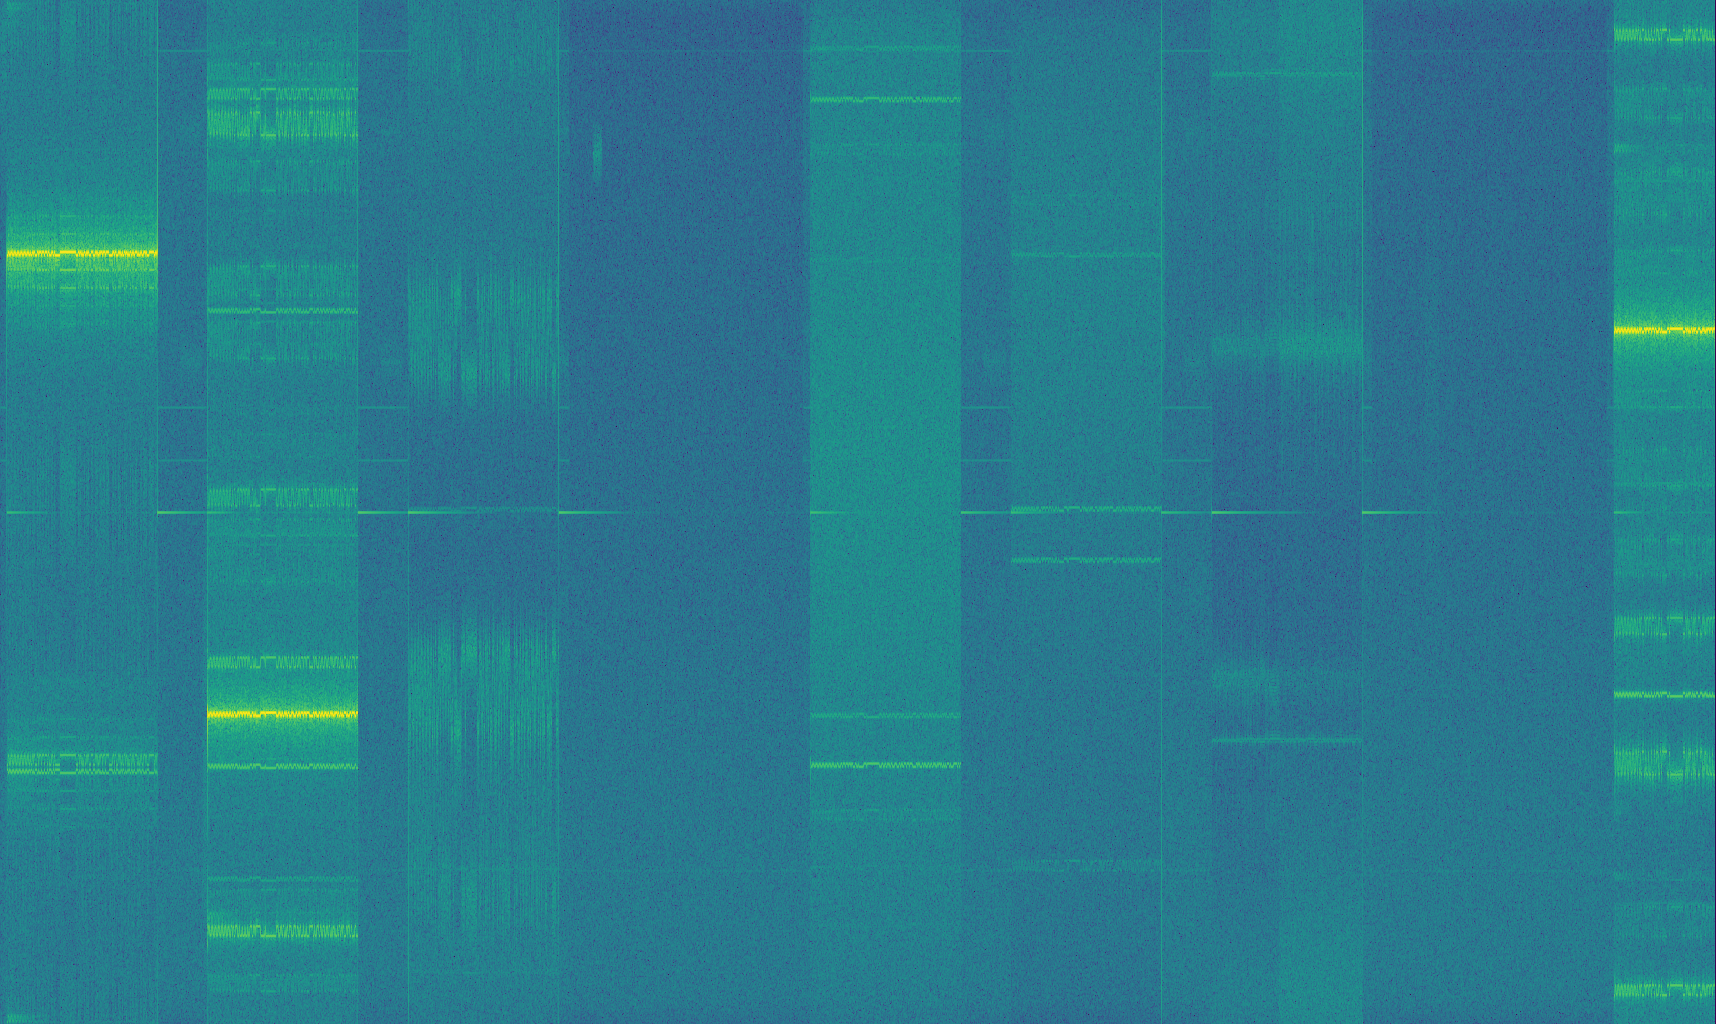
\includegraphics[width=\columnwidth]{FIGURES/cdrf/RadioMaster_TX16S_NA_2433_In_Cage_sample_170.png}
        \caption{RadioMaster TX16S}
    \end{subfigure}
\caption{Representative spectrograms from the CDRF dataset, illustrating the diversity of signal types and device behaviors captured during controlled data collection.}
\label{fig:spec}
\end{figure}

Next, we adjust the parameters on both the SDR devices and the UAVs to ensure they are properly aligned for optimal data recording quality. This includes settings such as the gain of the SDR device, the center frequency, and the bandwidth of the UAV's video transmission. In this work, we set the gain of the SDR device to 50 dB for indoor use and 76 dB for outdoor use, with a sampling rate of 20 MHz for both environments. For the video signal from UAVs, we select one of the channels in each of the frequency bands supported by the UAV, e.g., 900MHz, 2.4GHz, or 5.8GHz. Generally, we choose the channels that are not commonly occupied by other non-UAV wireless traffic in order to ensure the quality of the collected data. After the UAV transmission channel is defined, we tune the center frequency of the SDR device to align it to the UAV channel. This ensures that any UAV signals with a bandwidth less than or equal to 20MHz can be fully captured. In addition, this frequency alignment can help simplify the data preprocessing step for any research focusing on frequency domain representation of the signals, because the resulting transformation from the raw data, e.g., spectrogram, will contain a centralized UAV signal.

After that, we run the data recording script from the laptop for a predefined time duration, and the raw data is generated and stored in a \texttt{\{drone\_\allowbreak manufacturer\}\_\allowbreak\{drone\_\allowbreak model\}\_\allowbreak \{bandwidth\}\_\allowbreak\{drone\_\allowbreak center\_\allowbreak freq\}\allowbreak\_\allowbreak\{drone\_\allowbreak operation\_\allowbreak mode\}.dat} file along with all the predefined labels. In CDRF, we record the UAV manufacturer, model, center frequency of UAV signals, and bandwidth for each recording in the corresponding filename or directory name. 

Finally, we implement additional software scripts, including a signal playback module in GNU Radio, to load the raw data file, to review the validity of the recorded raw data, and to ensure the signals recorded match the predefined parameters. We also estimate the SNR and the channel condition to make sure the recorded signals are in a rather clean state. Fig.~\ref{fig:spec} shows some representative spectrograms from the CDRF dataset, illustrating device behaviors captured during controlled data collection. 

%%% new section on outdoor data collection %%%

\subsection{Collection of Outdoor Data}

To complement our controlled indoor recordings, we conducted extensive outdoor data collection sessions. This effort was aimed at enhancing the diversity and realism of the CDRF dataset by capturing UAV signals in complex RF environments, which better reflect real-world operational conditions with various signal sources and environmental factors.

For each outdoor session, we meticulously recorded a comprehensive set of metadata to ensure the data's utility and reproducibility. The raw I/Q data files are organized into a structured directory hierarchy where each directory name systematically encodes the key parameters of the recording session. The naming convention is as follows:

\texttt{\{device\}\_\allowbreak\{status\}\_\allowbreak\{env\}\_\allowbreak\{sdr\_gain\}\_\allowbreak\{splitter\}\_\allowbreak\{duration\_recording\}\_\allowbreak\{distance\}\_\allowbreak\{altitude\}\_\allowbreak\{center\_freq\}\_\allowbreak\{drone\_c\_freq\}\_\allowbreak\{bw\}\_\allowbreak\{snr\}\_\allowbreak\{sampling\_rate\}\_\allowbreak\{record\_dir\}.dat}

The fields in the directory name are defined as:
\begin{itemize}
    \item \texttt{device}: The model of the drone or device being recorded.
    \item \texttt{status}: The operational state of the drone (e.g., hovering, flying, on the ground).
    \item \texttt{env}: The environment where the recording took place.
    \item \texttt{sdr\_gain}: The receiver gain of the SDR in dB.
    \item \texttt{splitter}: A flag indicating if a signal splitter was used.
    \item \texttt{duration\_recording}: The total duration of the recording in seconds.
    \item \texttt{distance}: The horizontal distance from the receiver to the drone in meters.
    \item \texttt{altitude}: The altitude of the drone in meters.
    \item \texttt{center\_freq}: The center frequency of the SDR receiver in MHz.
    \item \texttt{drone\_c\_freq}: The drone's transmission center frequency in MHz.
    \item \texttt{bw}: The signal bandwidth in MHz.
    \item \texttt{snr}: The estimated SNR in dB.
    \item \texttt{sampling\_rate}: The sampling rate of the SDR in MHz.
    \item \texttt{record\_dir}: The name of the directory where the recording is stored.
\end{itemize}

Fig.~\ref{fig:outdoor_spec} presents a selection of representative spectrograms from our outdoor data collection, featuring signals from various drones such as the Autel EXOII, DJI Inspire1, DJI Mavic3, and DJI Phantom3 Advanced. In stark contrast to the clean, isolated signals captured indoors (as seen in Fig.~\ref{fig:spec}), these outdoor spectrograms exhibit significantly higher levels of background noise and interference. This is visually evident from the brighter and more cluttered appearance of the spectrogram backgrounds, a direct result of the complex real-world RF environments in which the data was collected. The inclusion of this noisier, more challenging data is crucial for developing and validating drone detection models that are robust enough for practical, real-world deployment.


\begin{figure}[!t]
    \centering
    \begin{subfigure}[h]{0.45\columnwidth}
        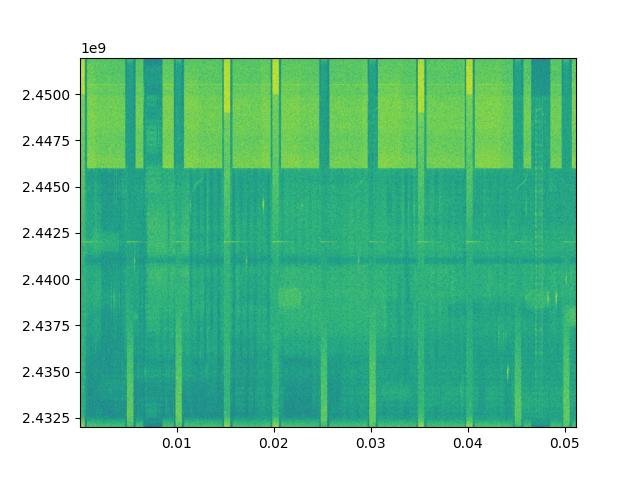
\includegraphics[width=\columnwidth, trim={2.2cm 1.5cm 1.8cm 1.5cm}, clip]{FIGURES/cdrf/outdoor/Autel-EXOII.jpg}
        \caption{Autel EXOII}
    \end{subfigure}
    \begin{subfigure}[h]{0.45\columnwidth}
        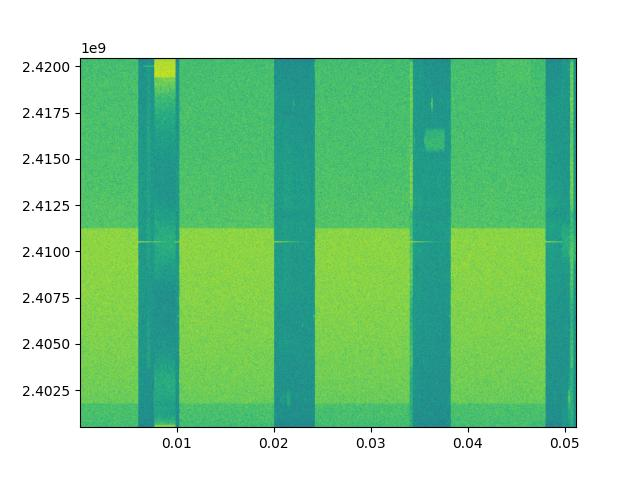
\includegraphics[width=\columnwidth, trim={2.2cm 1.5cm 1.8cm 1.5cm}, clip]{FIGURES/cdrf/outdoor/DJI-Inspire1.jpg}
        \caption{DJI Inspire1}
    \end{subfigure}
    \begin{subfigure}[h]{0.45\columnwidth}
        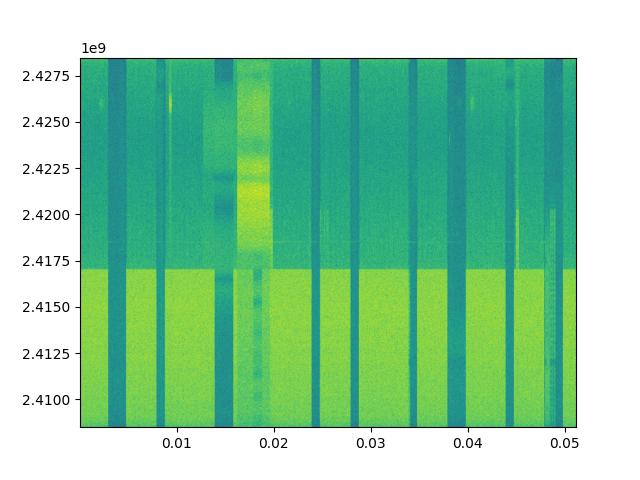
\includegraphics[width=\columnwidth, trim={2.2cm 1.5cm 1.8cm 1.5cm}, clip]{FIGURES/cdrf/outdoor/DJI-Mavic3.jpg}
        \caption{DJI Mavic3}
    \end{subfigure}
    \begin{subfigure}[h]{0.45\columnwidth}
        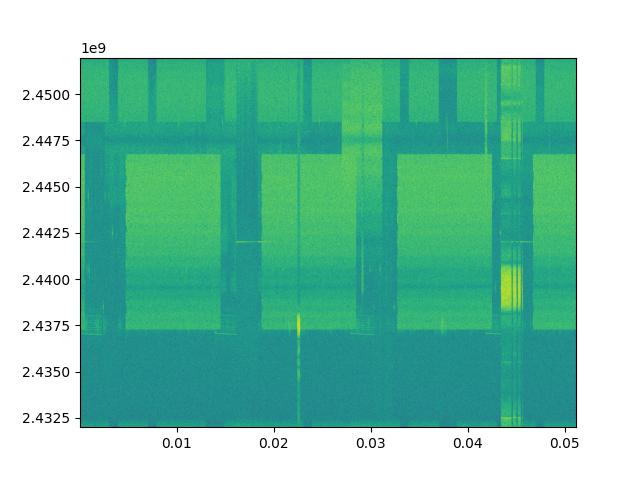
\includegraphics[width=\columnwidth, trim={2.2cm 1.5cm 1.8cm 1.5cm}, clip]{FIGURES/cdrf/outdoor/DJI-Phantom3Adv.jpg}
        \caption{DJI Phantom3 Advanced}
    \end{subfigure}
\caption{Representative spectrograms from the outdoor dataset, showcasing the variability in signal characteristics due to environmental factors.}
\label{fig:outdoor_spec}
\end{figure}



\subsection{Dataset Composition and Signal Characteristics}
The CDRF dataset is designed to provide a comprehensive and diverse collection of RF signals for drone detection and identification research. The dataset is built upon a large corpus of raw signal captures, totaling approximately 500+ GB of raw data.

At the core of our dataset is a significant diversity of drone models and signal types. The collection includes signals from 39 unique classes, encompassing 23 distinct commercial and hobbyist UAV models, their remote controllers, and operational variants (e.g., armed vs. unarmed states). This variety, spanning major manufacturers such as DJI, Autel, and Parrot, ensures that models trained on CDRF are exposed to a wide range of communication protocols, a substantial leap from the handful of models found in many previous datasets. In addition to drone signals, we include a substantial number of ``no-drone" recordings, capturing ambient RF noise and other common interferers like Wi-Fi signals. This enables the training of robust binary classifiers that can distinguish between the presence and absence of drone activity, a critical requirement for real-world deployment. To further challenge detection and identification algorithms, the dataset also contains recordings of multiple drones operating simultaneously in the same airspace.

All raw data is stored using the In-phase and Quadrature (I/Q) sampling method. Each sample is represented as an interleaved binary bitstream of two 32-bit floating-point numbers, capturing the full complex signal. This raw format is crucial as it allows researchers to develop and test novel signal processing and feature extraction techniques that operate directly on the baseband signal, prior to any transformations like the STFT.

% \todo[inline, color=yellow!40]{AeroDefense Team: Did I get this right}
% \todo[inline, color=blue!40]{I recommend just say something like: "In contrast, signals used for video transmission typically have wider bandwidth and longer duration than control signals." You can also mention that the controller signals are usually very narrowband signals somewhere earlier in this paragraph if needed.}
% \todo[inline, color=blue!40]{It will be not that appropriate to say the drone signal is transmitted on a "fixed" channel. A better word will be needed here, maybe "predefined"? It is generally something that the pilot can have more control on by selecting the channels where to transmit the video signals. Meanwhile there isn't such flexibility for transmitting the controller signals.}
The signals captured in CDRF exhibit a variety of characteristics typical of modern drone communication systems. Many of the drones utilize Frequency-Hopping Spread Spectrum (FHSS) for their command and control links. These signals are defined by key parameters such as their hopping frequency, duration, duty cycle, and the period of their hopping pattern. In contrast, signals used for video transmission typically have wider bandwidth and longer duration than control signals. We define the collection of these characteristics as the RF Drone Fingerprint, which serves as a rich input for deep learning models to differentiate between drone types.

Furthermore, our data captures the inherent behavioral variability of drone signals. For instance, the frequency hopping patterns of a drone during its initial pairing process can differ significantly from those during normal flight operations. The dataset also captures more subtle phenomena, such as the variable time duration of video transmission signals from certain drone models, a characteristic that can serve as another important feature for robust classification.


\section{Data Preprocessing, Augmentation, and Annotation}
\label{sec:data_processing}

We release both a raw-signal processing pipeline and augmentation utilities designed to create realistic, label-consistent training data from complex I/Q captures. All components are open-source and parameterized for reproducibility.

\subsection{Spectrogram Generation}
Raw complex I/Q streams are transformed into time–frequency representations via the STFT. Given a complex signal $x[n]$, window $w[n]$, window length $N$, and hop size $H$, the STFT is ~\cite{oppenheim1999discrete}
\[
X(m,k) \;=\; \sum_{n=0}^{N-1} x[n+mH]\; w[n]\; e^{-j 2\pi kn/N},
\]
where $m$ is the discrete time index and $k$ is the discrete frequency index.

We compute the power spectrogram $S(m,k) = \lvert X(m,k)\rvert^2$ and render in dB as
\[
S_{\mathrm{dB}}(m,k) \;=\; 10\log_{10}\big(S(m,k)+\epsilon\big),
\]
where $\epsilon$ represents a very small, positive constant used to avoid taking the logarithm of zero. After that map to RGB using a perceptual colormap. By default, we use \texttt{scipy.signal.stft}~\cite{virtanen2020scipy} with a Hann window, $N=\texttt{FFT\_SIZE}=1024$, overlap $=128$ samples, and return two-sided spectra with DC centered via \texttt{fftshift}. Default sampling is $\texttt{SAMPLING\_RATE}=20$\,MHz and we generate $\texttt{NUM\_FFT\_SPEC}=1500$ time bins per sample. Spectrograms are exported as PNG images alongside per-sample metadata.

\subsection{Frequency Resolution and Colormap Selection}
The window size $N$ and hop $(N-\text{overlap})$ set the time–frequency trade-off; larger $N$ improves frequency resolution at the cost of temporal precision. All parameters are exposed to support ablations. We provide multiple colormaps (\texttt{viridis}, \texttt{plasma}, \texttt{inferno}, \texttt{magma}, \texttt{cividis}, \texttt{gray}, \texttt{hot}) to test color sensitivity; the default pipeline normalizes spectrograms to $[0,1]$ before colorization and composites to RGB for consistent rendering.

\subsection{Data Normalization}
We include signal-level and spectrogram-level normalization operators:
\begin{itemize}
    \item \emph{Power normalization} of complex I/Q to unit average power: $\tilde{x}=x/\sqrt{\mathbb{E}\lvert x\rvert^2+\epsilon}$.
    \item \emph{Z-normalization} of real and imaginary parts independently to zero mean, unit variance.
    \item \emph{Spectrogram normalization} options: per-frequency z-score, per-time z-score, or global min–max to $[0,1]$ prior to colorization.
\end{itemize}

These are selectable in the augmentation scripts and can be toggled per experiment.

\begin{figure*}[htbp]
    \centering
    \begin{subfigure}[h]{0.6\columnwidth}
        \centering
        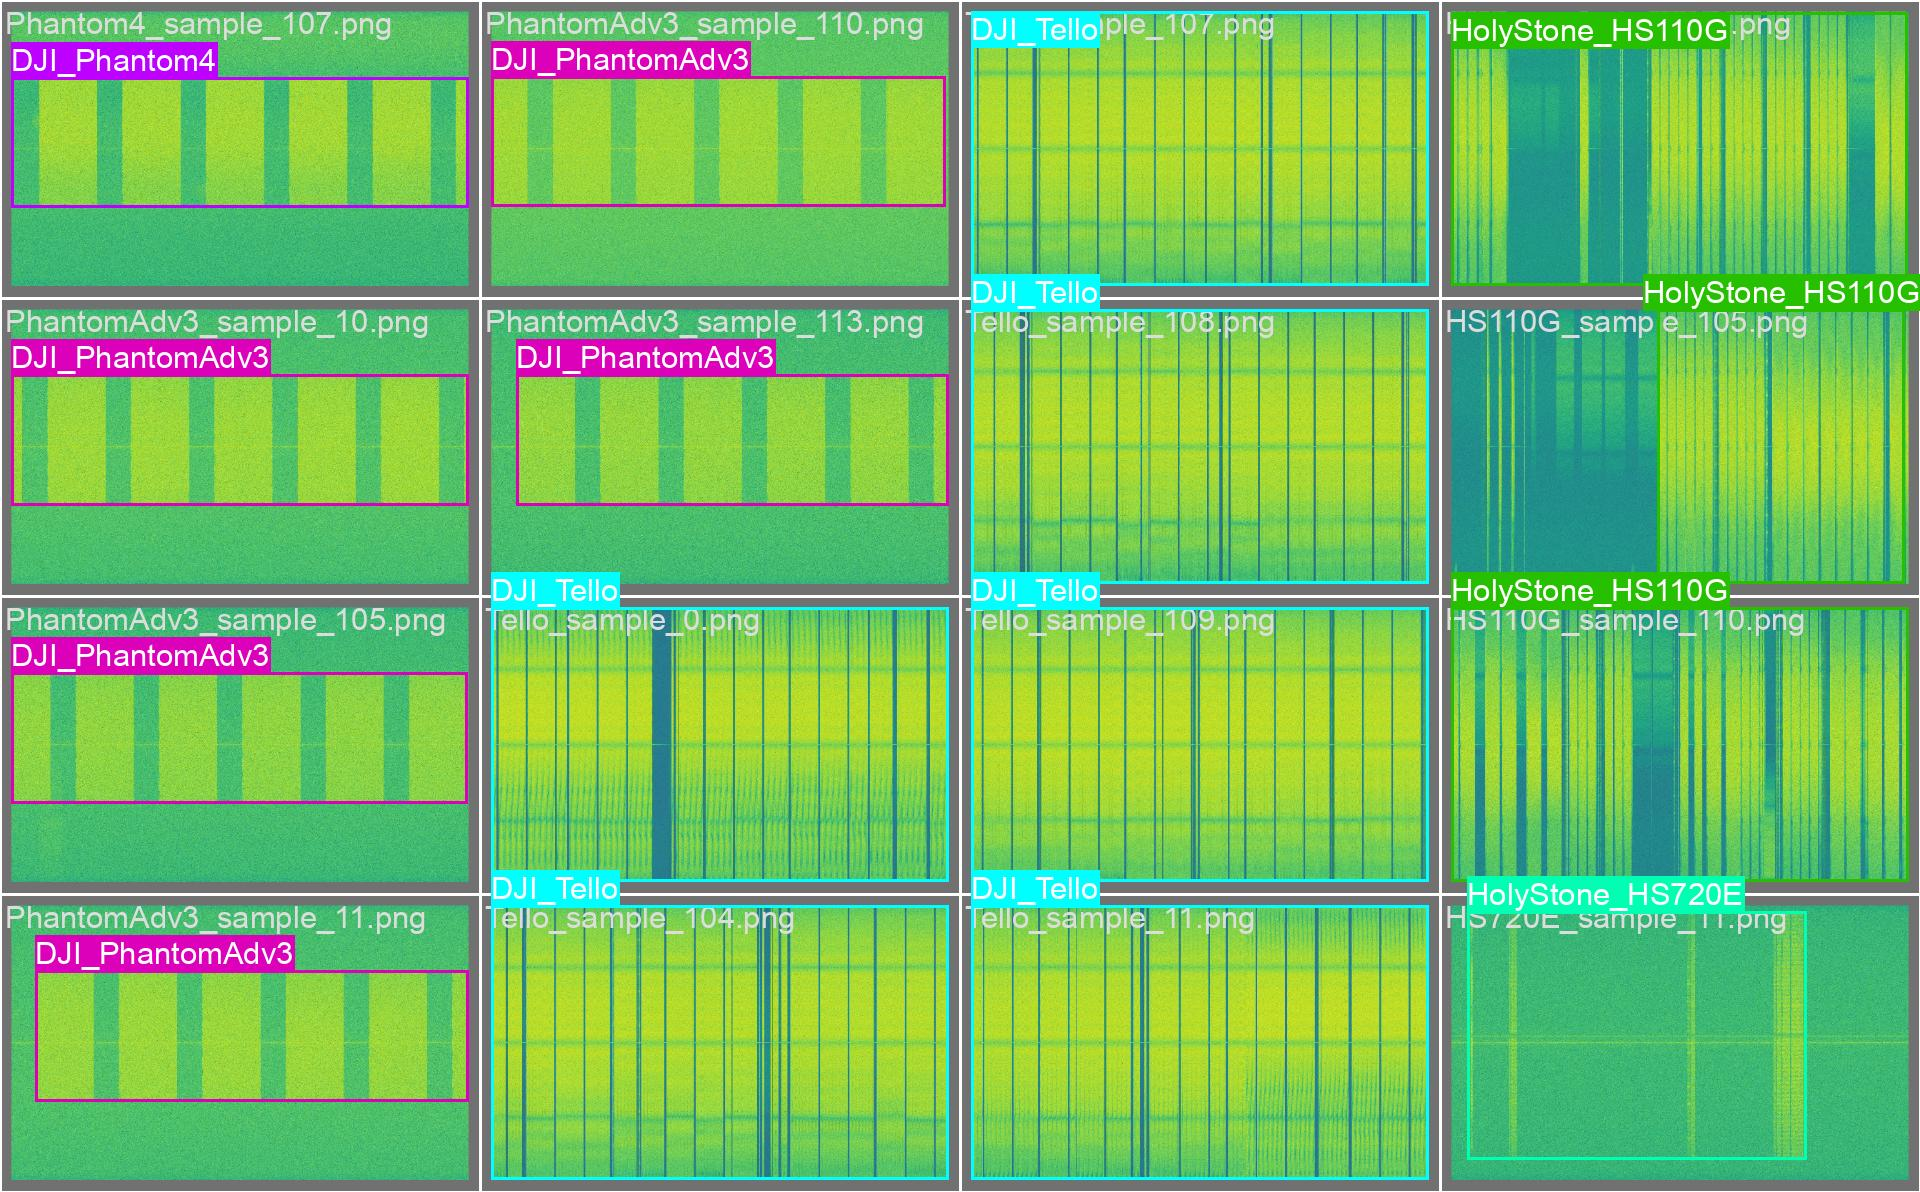
\includegraphics[width=\columnwidth]{FIGURES/cdrf/val_batch1_labels.jpg}
        \caption{Annotated Data.}
    \end{subfigure}
    \begin{subfigure}[h]{0.6\columnwidth}
        \centering
        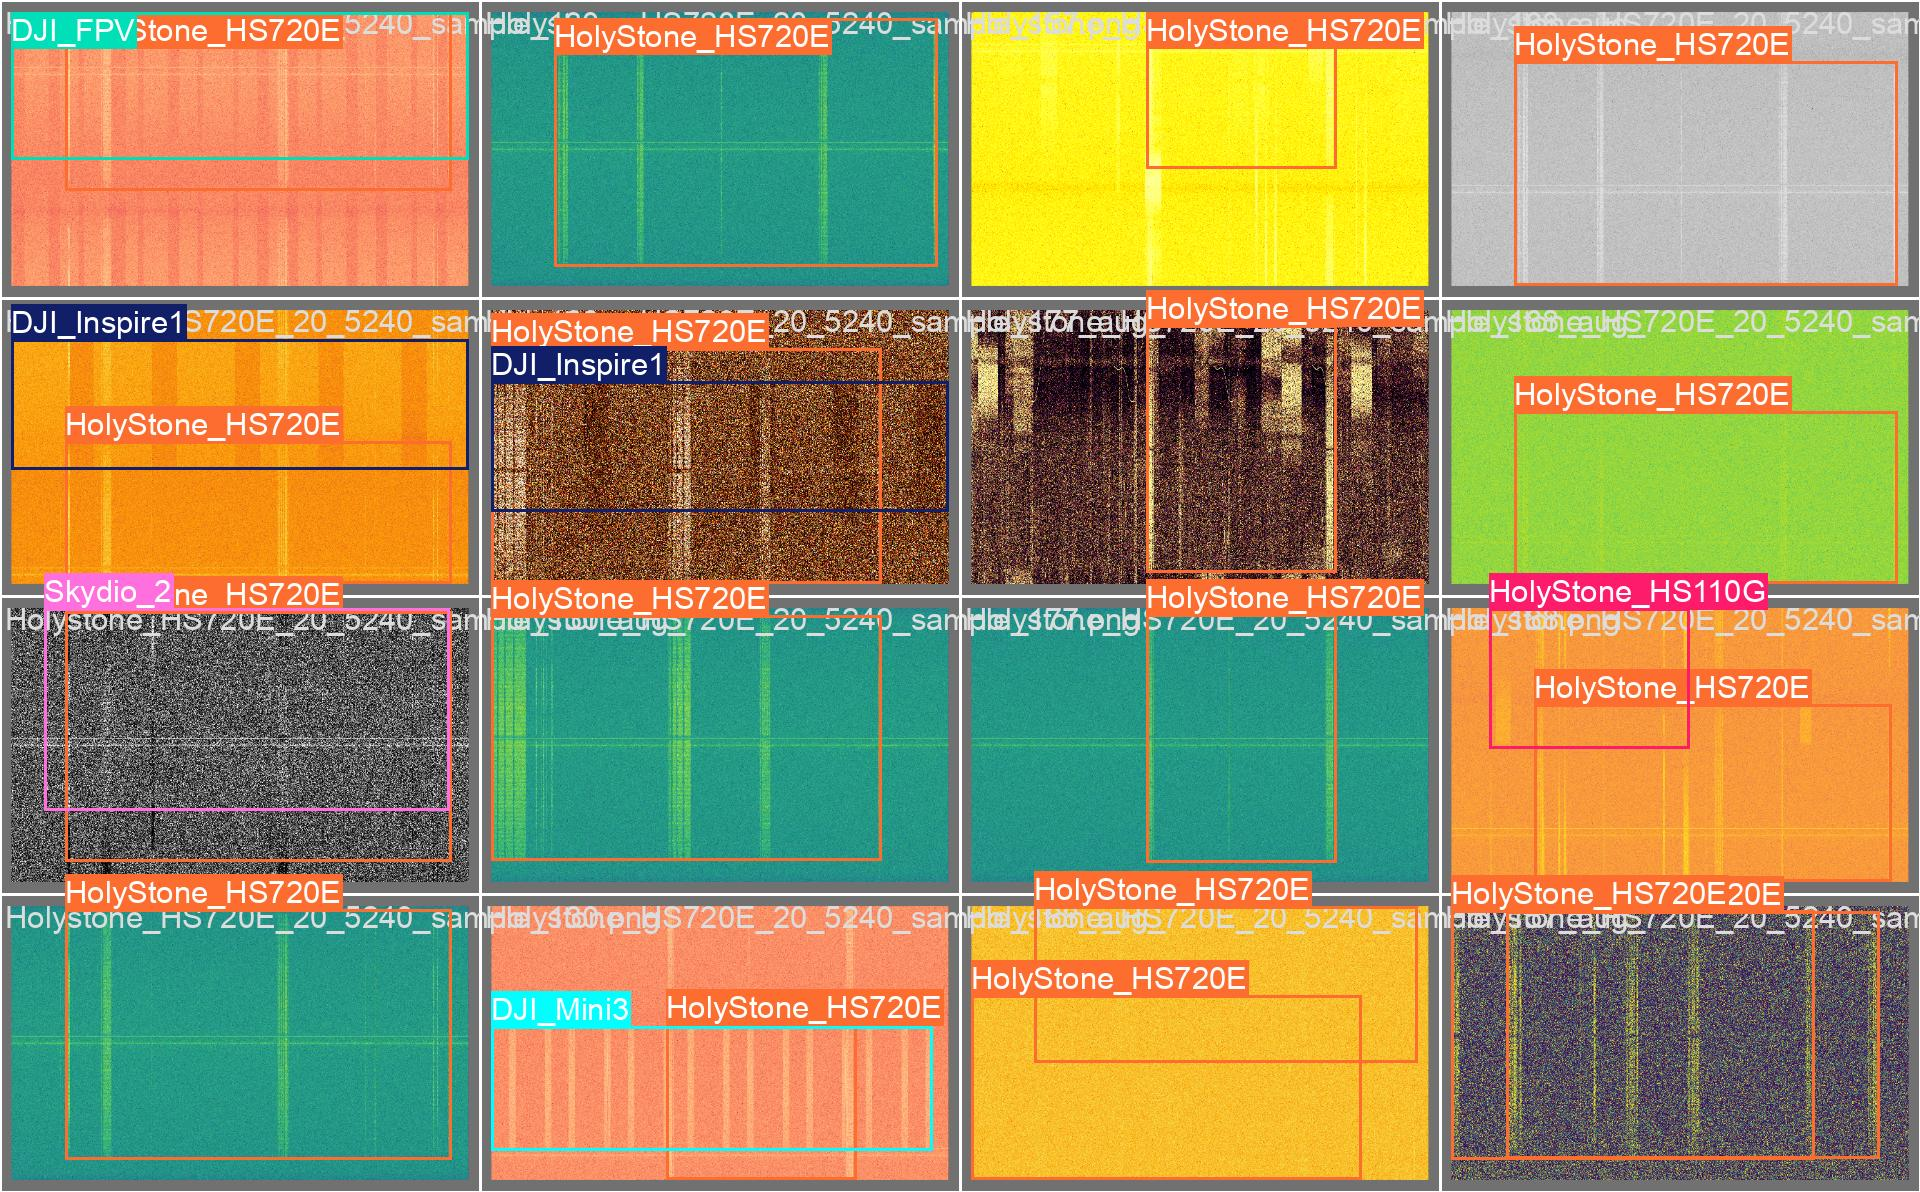
\includegraphics[width=\columnwidth]{FIGURES/cdrf/val_batch3_labels.jpg}
        \caption{Augmented Data.}
    \end{subfigure}
    \caption{Examples of annotated and augmented data.}
    \label{fig:augmented_data}
\end{figure*}

\subsection{Custom Augmentation Tools}
Our augmentation operates at the \emph{raw-signal} (I/Q) level to better preserve RF physics and then projects to spectrograms, with exact label propagation to detection annotations.

\subsubsection{SNR Conditioning via AWGN}
To synthesize controlled SNRs, we add complex AWGN $n\sim\mathcal{CN}(0,\sigma^2)$ to $x$ where the noise power $\sigma^2$ is chosen for target $\mathrm{SNR}_{\mathrm{dB}}$:
\[
P_s=\mathbb{E}\lvert x\rvert^2,\quad \mathrm{SNR}_{\mathrm{lin}}=10^{\mathrm{SNR}_{\mathrm{dB}}/10},\quad\sigma^2=P_s/\mathrm{SNR}_{\mathrm{lin}}.
\]  

We optionally export noise-only spectrograms for analysis and create SNR-stratified dataset variants (e.g., per-SNR subdirectories), enabling robustness sweeps.

\subsubsection{Frequency Shifting}
We simulate carrier offsets and front-end errors by multiplying with a complex exponential
\[
x_{\Delta f}[n] \;=\; x[n]\; e^{j2\pi \Delta f \, n/F_s},
\]
which induces a vertical translation on the spectrogram and where $F_s$ is sampling rate. This is applied before STFT and is label-consistent with our detection annotation recomputation (below).

\subsubsection{Interferer Mixing}
To emulate spectrum crowding, we mix two normalized signals at a controllable ratio $\alpha\in[0,1]$:
\[
x_{\text{mix}} \;=\; \operatorname{norm}\big(x_1\;+\;\alpha\, x_2\big),
\]
optionally with independent frequency shifts on each source. This produces realistic co-channel scenarios directly in the I/Q domain.

\subsubsection{Spectrogram Rendering Variants}
Augmented samples are rendered under randomized, but reproducible, choices of colormap and normalization policy to increase visual diversity while keeping frequency content intact.

\subsubsection{Background Noise and Non-Target Signals}
Our dataset includes a comprehensive corpus of non-target signals, captured from diverse environments where no drones were active. To facilitate common machine learning workflows, we provide a suite of tools to extract these ``no-drone" segments and generate unified metadata files for mixed-signal experiments. This curated collection of real-world negative samples is crucial for training well-calibrated binary detectors and is explicitly designed to support advanced strategies like hard-negative mining.

\subsection{Annotation Strategy}
We adopt YOLO-format annotations on spectrogram images with a \emph{whole-signal} policy: contiguous RF emission bursts from a device are annotated as a single object to capture both spectral morphology and temporal occupancy. Fig.~\ref{fig:augmented_data} shows examples of annotated data and augmented data with annotations.

In general, a spectrogram of a UAV signal segment consists of a sequence of ON-OFF states, which represents the transmission pattern of the UAV in both time and frequency domain. In order to lead YOLO model to better capture the signal characteristics in both domains, we define the annotation policy as that, the bounding box for each type of signals in a spectogram image will start and end with an ON state of the signal. The OFF states at the beginning and end of a spectrogram are neglected. This can help the YOLO model to track the start and end of a transmission, and thus to output more accurate bounding boxes. Meanwhile, if the RF emission bursts captured by a spectrogram are with limited time duration, i.e., $<10\%$ of the time duration of the spectrogram, or there is only a single ON state in the whole spectrogram, no bounding box annotation will be given, and the spectrogram image will be labeled as background in those cases. 

As for the RC signals, due to its frequency-hopping property, in CDRF we aim at providing two types of YOLO-formated annotation to support the flexibility of future research or implementation in potentially different purposes. 
\begin{itemize}
    \item We provide one bounding box covering all the RC signal bursts captured in a spectrogram. Similar to the UAV signal labeling, we ensure that the edges of the bound box align with the start and end of the sequence of RC signal bursts
    \item CDRF also contains annotation for RC signal bursts transmitted at the same channel. Since the frequency-hopping behavior is not guaranteed to occur or being captured in every single spectrogram in a continuous raw data recording, we believe that this type of annotation can contribute the learning of YOLO models and improve the detection performance when deploying it in reality. 
\end{itemize}

Moreover, due to the fact that most of the RC signals are narrowband and in short duration for each ON state, we do not provide any bounding box annotation to the spectrogram that contains only one single ON state. The reason behind this design choice for annotation strategy is that the bound box covering only single ON state does not provide any information for the model to learing about its pattern across either time or frequency domain. Similar statement on UAV video signal annotation is also demonstrated in \cite{nelega2023radio}. Also, the detection or classification based on a single ON state is generally neither expected nor considered reliable in real-world UAV detector deployment scenarios.

\subsubsection{Label-Preserving Transforms with Wrap-Around}
Frequency shifts correspond to vertical translations in normalized image coordinates by $\Delta y=\Delta f/F_s$. We recompute bounding boxes analytically after augmentation and correctly handle wrap-around at the top/bottom edges: if a box straddles the boundary after shift, it is split into two valid boxes whose heights sum to the original. Boxes are also filtered by a configurable minimum height to avoid degenerate labels after extreme shifts.

\subsubsection{Dataset Hygiene and Third-Party Integration}
We include utilities to normalize third-party releases (e.g., Roboflow-style layouts) into a consistent hierarchy (\texttt{images/}\,\,\texttt{labels/} with class folders and \{train,val,test\} splits) and to preserve class mappings. This enables direct augmentation and training across heterogeneous sources.

\subsection{Reproducibility and Metadata}
Each sample carries rich metadata to ensure reproducibility: original file path, device/model label, sampling rate, FFT size, number of STFT frames, per-sample time bounds (start/end in seconds), center frequency, and output paths for spectrograms. All processing parameters (e.g., window size, overlap, SNR target, shift amounts, mixing weights) are saved or deterministically re-creatable from configuration, facilitating exact regeneration of training splits and ablation studies.

\section{Machine Learning Tasks and Baselines}
\label{sec:ml_tasks}
This section details the machine learning tasks supported by our dataset, the baseline models implemented, and their performance. We address drone detection, single-label classification, multi-label classification, open-set recognition, and hierarchical classification.

\subsection{Drone Detection (YOLO)}
\label{subsec:yolo_experiments}

\subsubsection{Task Definition}
Given a time–frequency spectrogram, the goal is to detect and localize RF emissions attributable to drones. The detector predicts a set of axis-aligned bounding boxes with class labels in YOLO normalized coordinates, where each object corresponds to a contiguous emission burst (whole‑signal policy) on the spectrogram.

\subsubsection{Baseline Model Architecture and Training}
We use a single-stage object detector, \texttt{YOLOv11n}~\cite{khanam2024yolov11} (Ultralytics~\cite{jocher2022ultralytics} v8.3.156), trained on spectrograms produced by our pipeline (\cref{sec:data_processing}). We evaluate two scenarios: (i) Clean, in which spectrograms are generated without augmentation; and (ii) Augmented, in which raw complex I/Q are transformed before STFT via frequency shifting, interferer mixing, and SNR conditioning. Models are initialized from COCO-pretrained weights~\cite{lin2014microsoft,jocher2022ultralytics,khanam2024yolov11}, trained with deterministic seeds, and validated at each epoch. Labels follow the whole‑signal policy, and for frequency shifts we recompute YOLO annotations exactly with wrap‑around handling on the frequency axis to preserve label consistency. Unless otherwise specified, Ultralytics defaults are used for input size, data augmentation, and non‑max suppression.

\subsubsection{Evaluation Metrics}
We report standard detection metrics: class-aggregated Precision and Recall; mean Average Precision at IoU 0.5 (mAP@0.5); and COCO-style mAP averaged over IoU thresholds from 0.5 to 0.95 in steps of 0.05 (mAP@[.5:.95]). For qualitative error analysis, we also include normalized confusion matrices computed from matched detections.

\subsubsection{Experimental Results and Baseline Performance}
% \todo[inline,color=blue!40]{Maybe Update the results using the latest augmentation and dataset to close the gap between the code and the paper; also the task has become more challenging over time so better performance and harder task is represented in the paper}
\begin{table}[hht]
\centering
\caption{YOLO detection results.}
\label{tab:yolo_detection_results}
\resizebox{0.8\linewidth}{!}{%
\begin{tabular}{lcccccc}
\toprule
Run & Epochs & Precision & Recall & mAP@0.5 & mAP@[.5:.95] \\
\midrule
Clean & 100 & 0.932 & 0.982 & 0.986 & 0.948\\
Augmented & 50 & 0.940 & 0.855 & 0.935
& 0.838\\
\bottomrule
\end{tabular}%
}
\end{table}

Table~\ref{tab:yolo_detection_results} summarizes the best validation checkpoints: The model trained without any augmentations (referred to as ``clean") achieves strong performance (Precision $=0.932$, Recall $=0.982$, mAP@0.5 $=0.986$, mAP@[.5:.95] $=0.948$), with the top mAP@[.5:.95] observed near epoch~78. Under augmentation, precision is maintained and slightly improved (Precision $=0.940$) while recall drops (Recall $=0.855$), yielding lower top‑line mAP (mAP@0.5 $=0.935$, mAP@[.5:.95] $=0.838$; best near epoch~49). This reflects the expected precision–recall trade‑off when training on harder, low‑SNR and interferer‑rich conditions: the detector becomes more conservative (fewer false positives) at the expense of increased misses (more false negatives). 

Despite this shift, the normalized confusion matrices in Fig.~\ref{fig:yolo_confusions} remain strongly diagonal for both regimes, indicating that whole‑signal annotations preserve class separability even under frequency shifts and spectrum crowding. The dominant degradation under augmentation is recall (missed detections) rather than systematic label confusion, suggesting room for robustness gains via longer training, class‑balanced sampling, or stronger backbones without altering the annotation policy.

\begin{figure*}[htbp]
    \centering
    \begin{subfigure}[h]{0.48\textwidth}
        \centering
        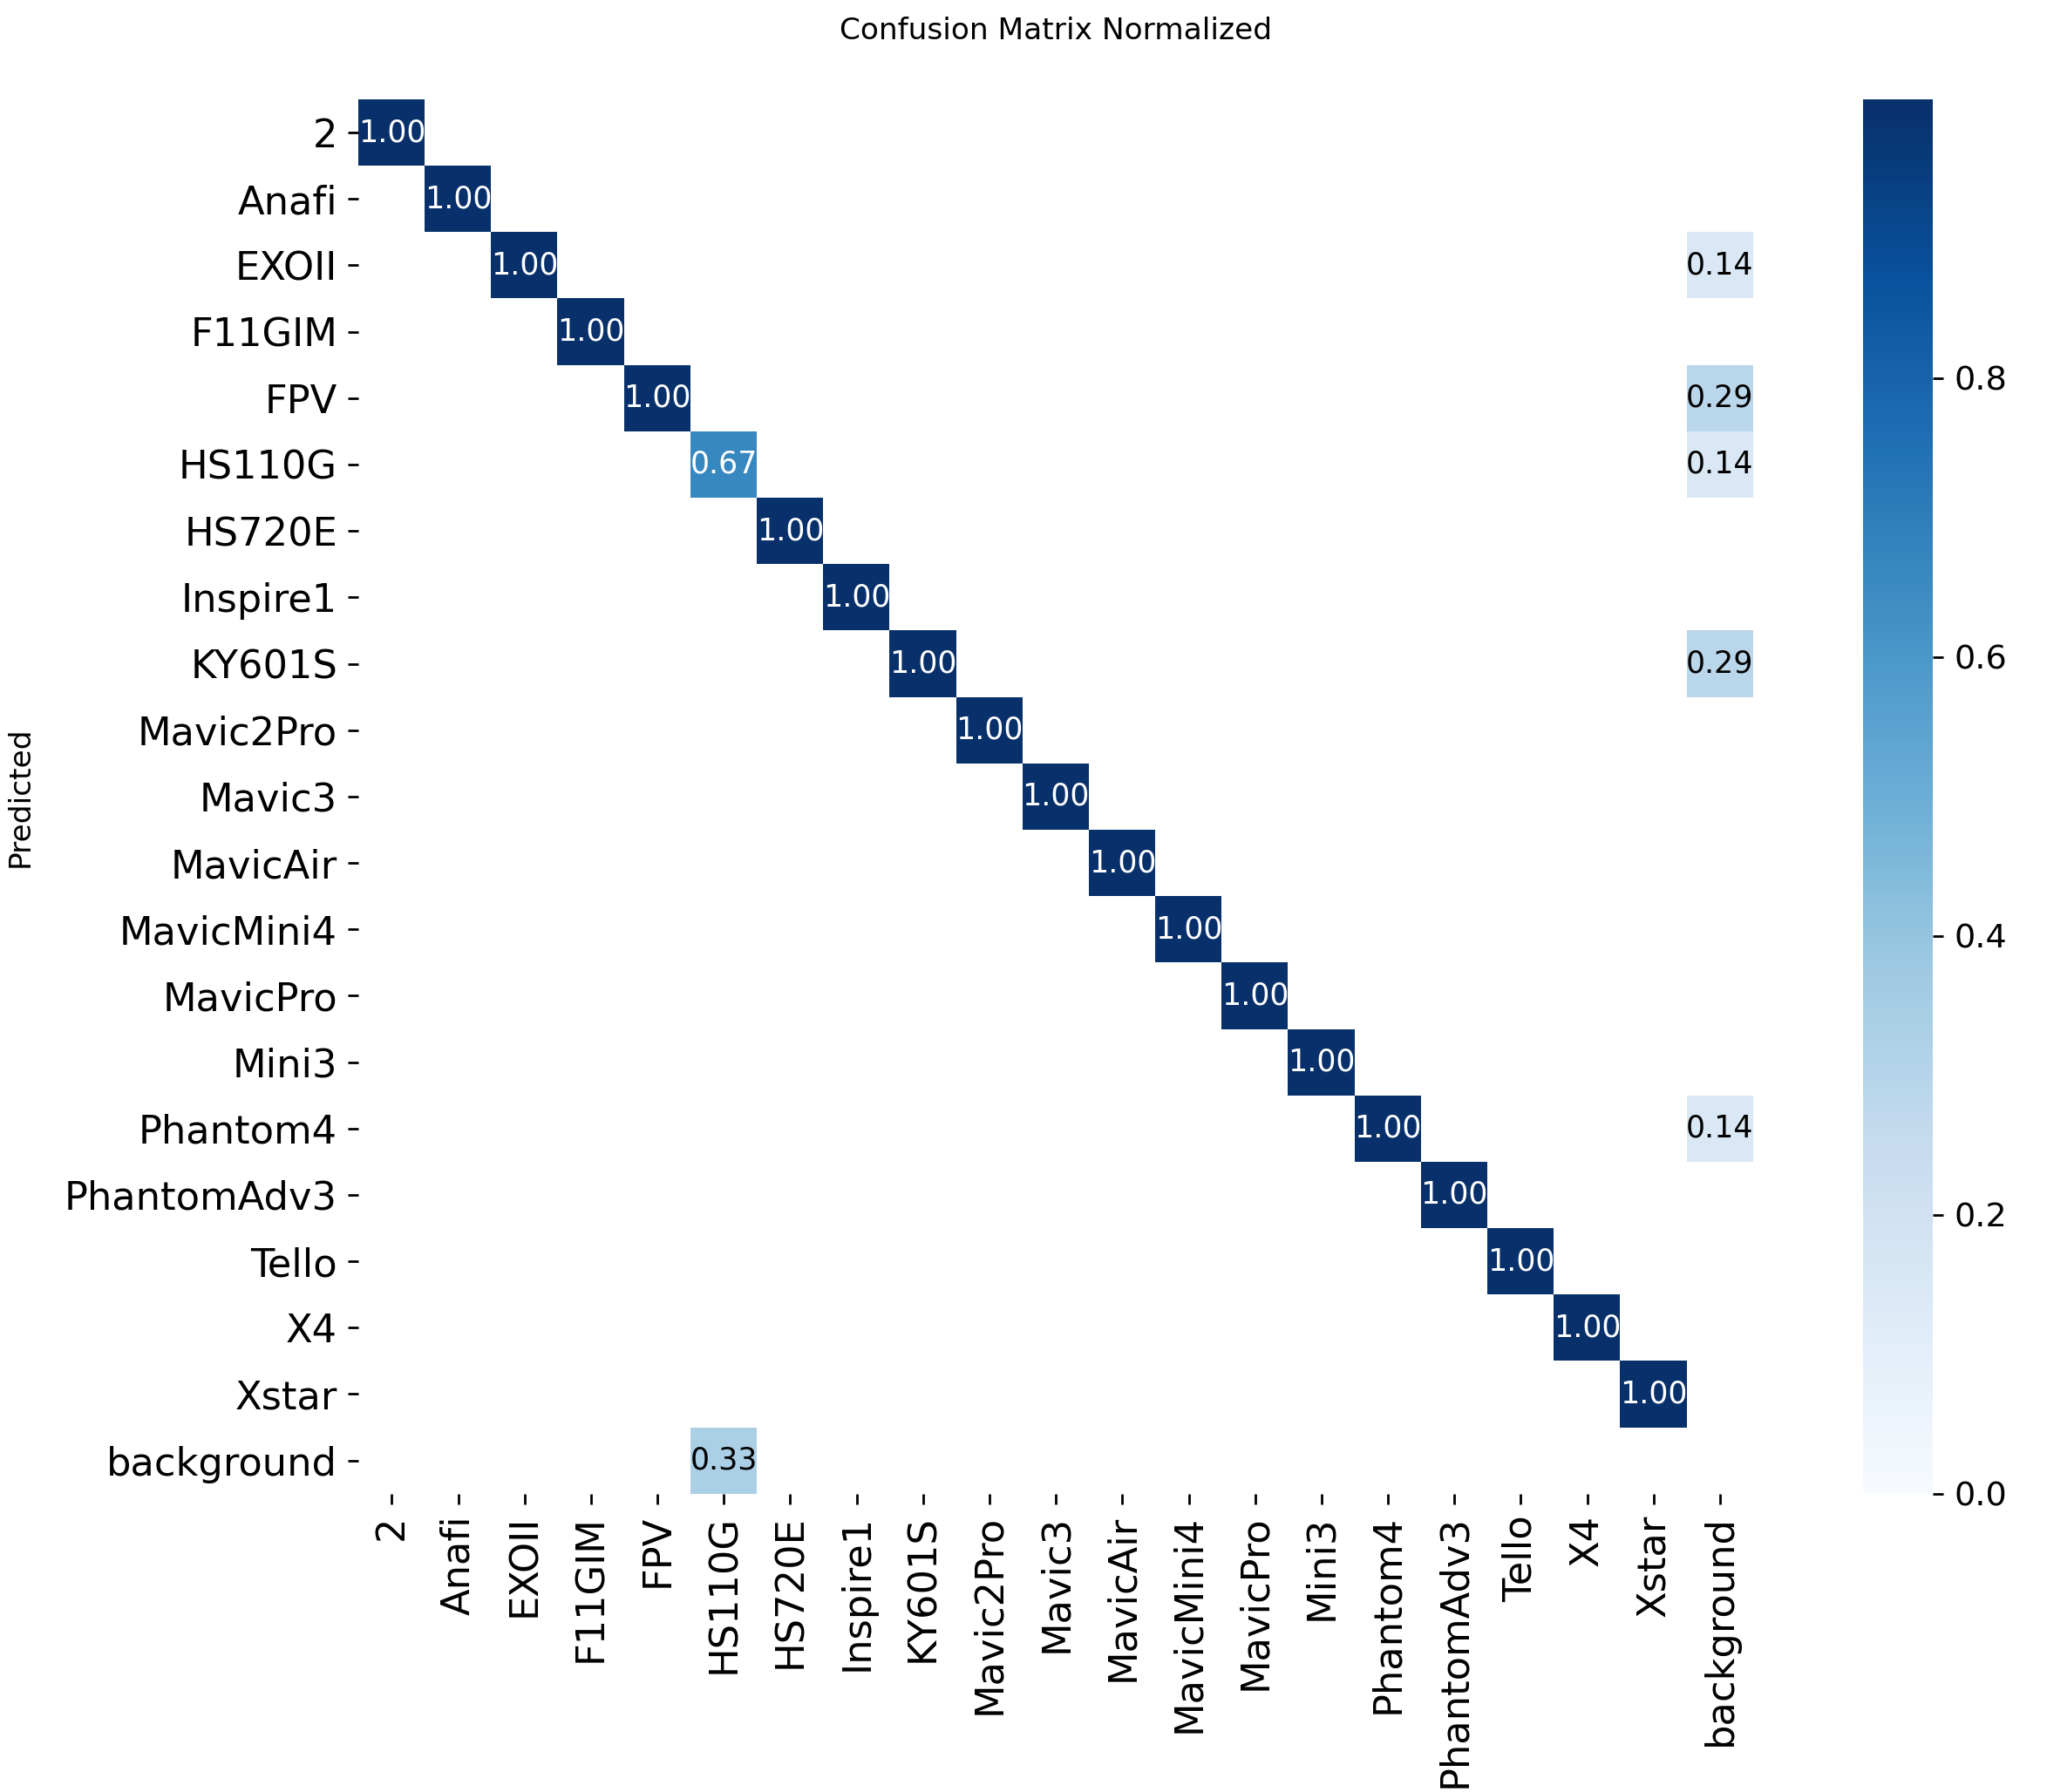
\includegraphics[width=\linewidth]{FIGURES/cdrf/clean_confusion_matrix_normalized.png}
        \caption{Clean: normalized confusion.}
    \end{subfigure}
    \hfill
    \begin{subfigure}[h]{0.48\textwidth}
        \centering
        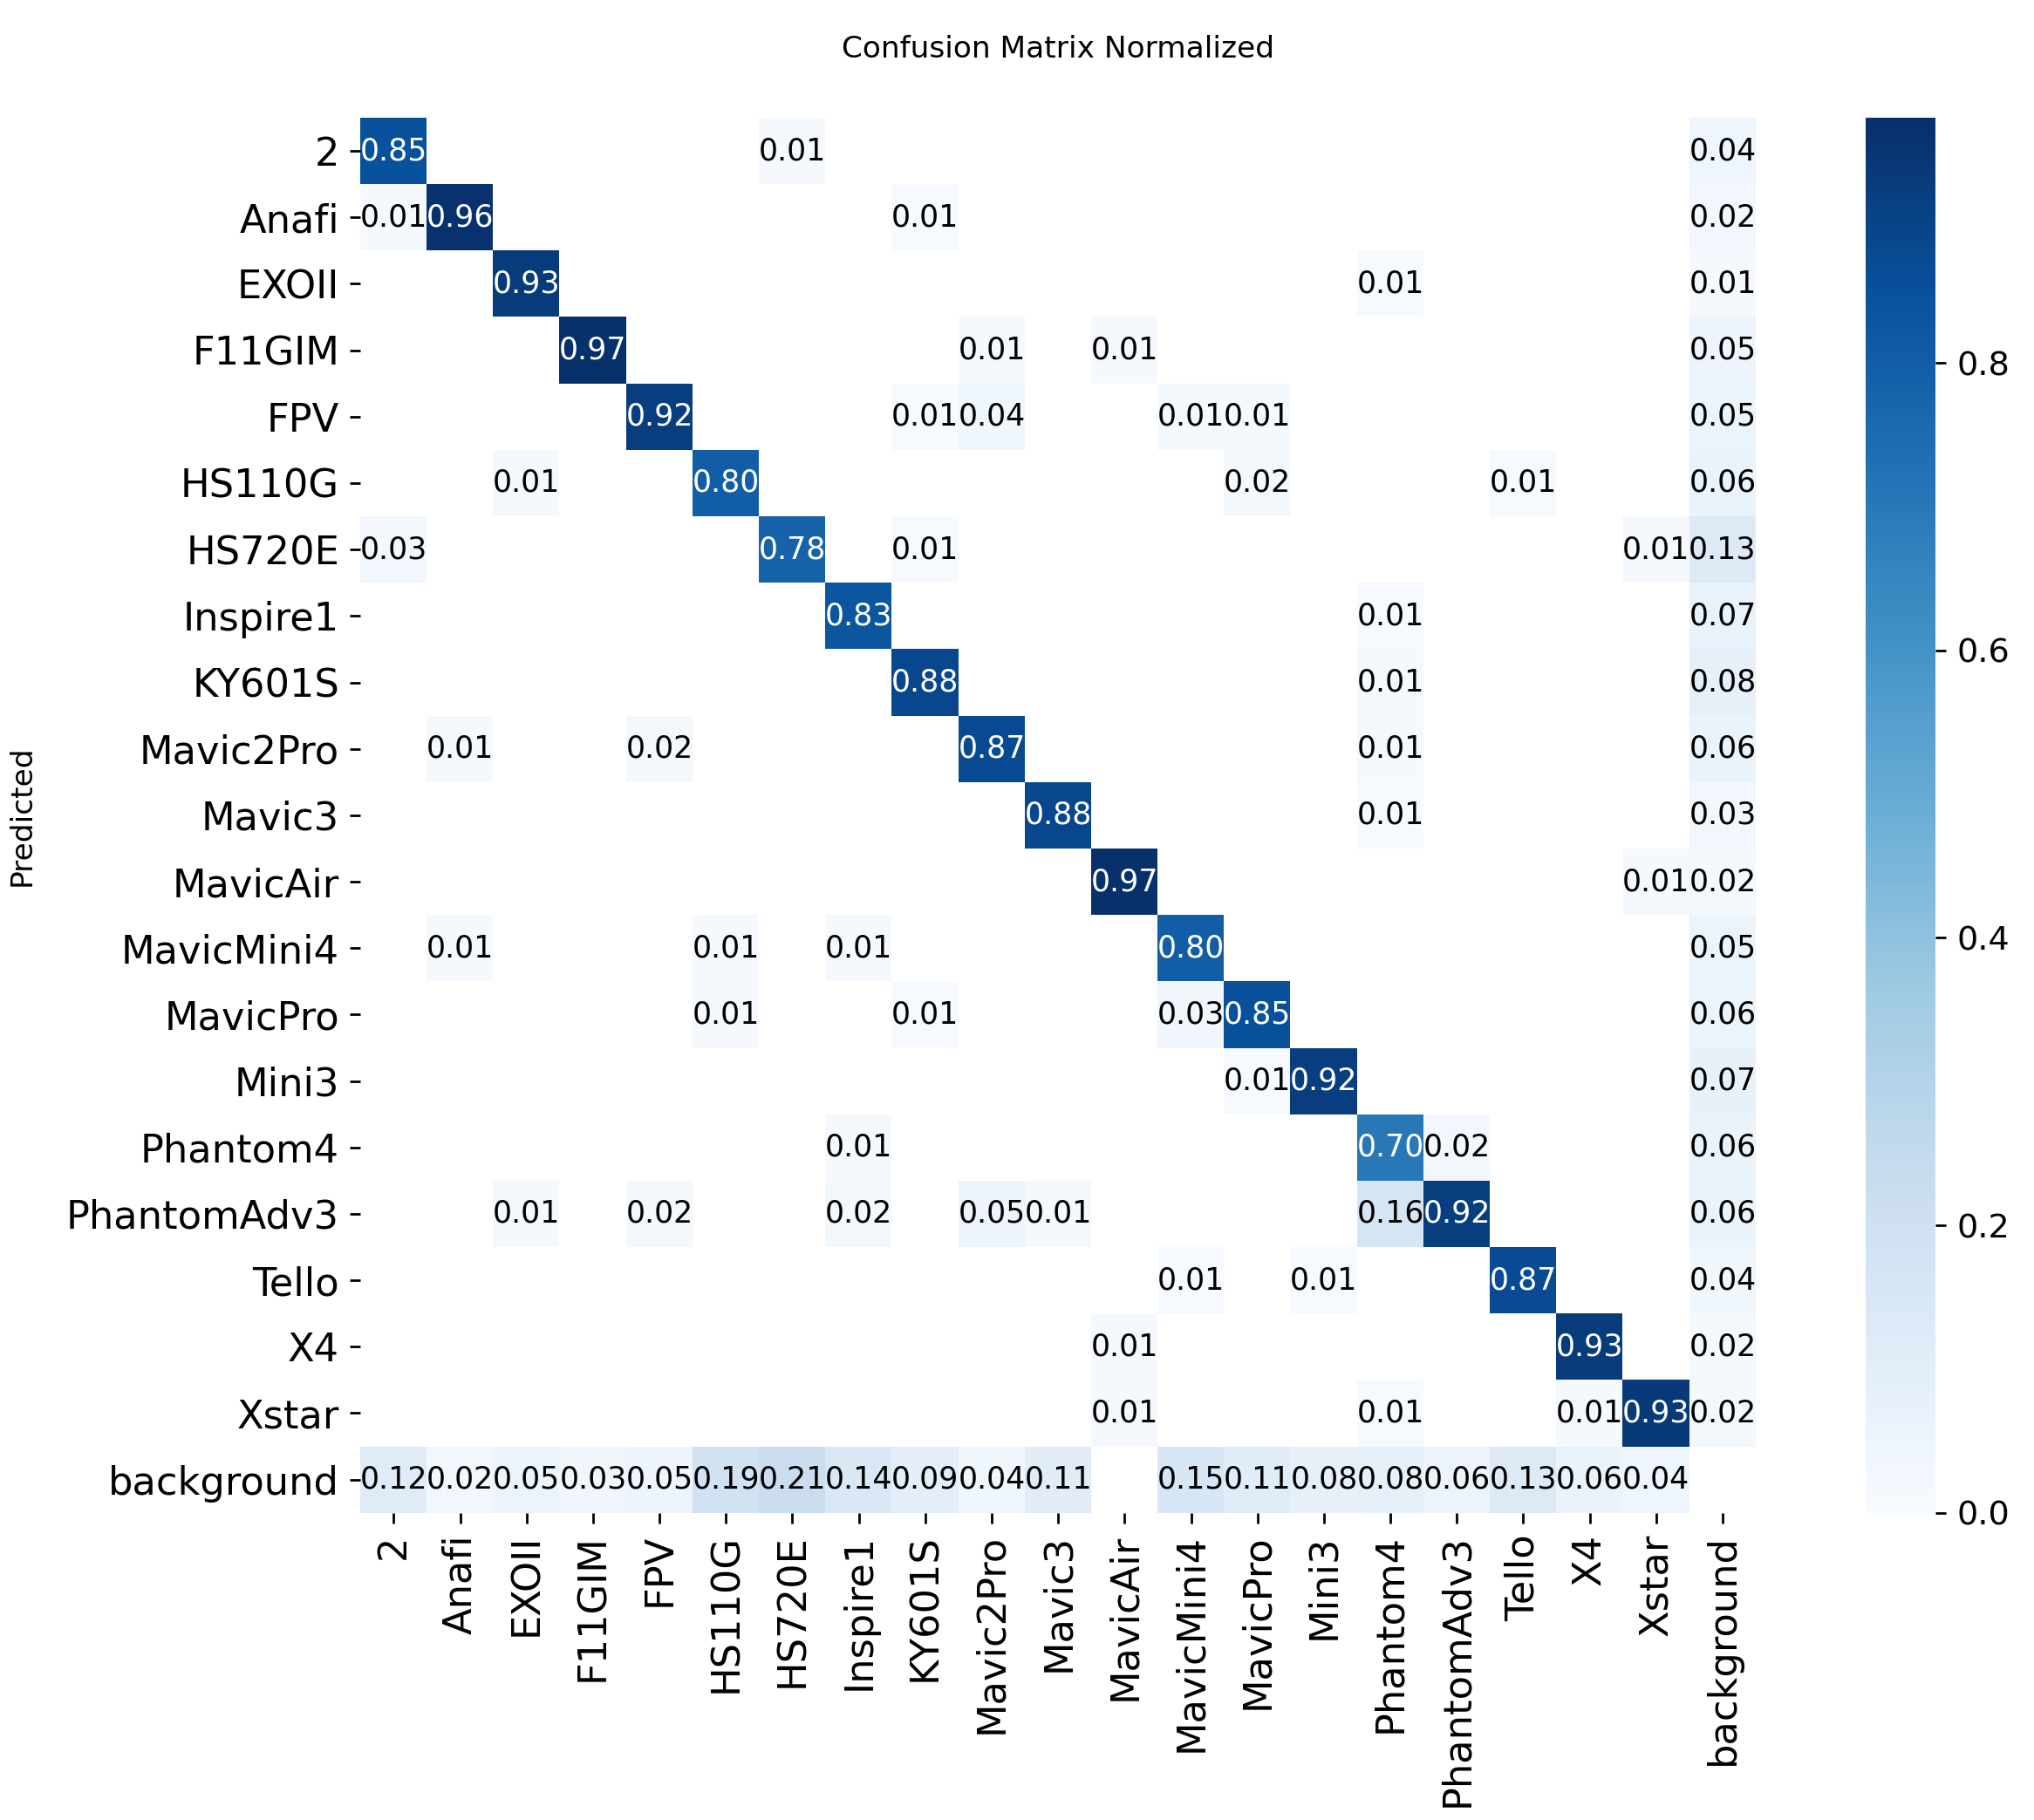
\includegraphics[width=\linewidth]{FIGURES/cdrf/augmented_confusion_matrix_normalized.png}
        \caption{Augmented: normalized confusion.}
    \end{subfigure}
    \caption{Class‑wise performance and error structure on validation.}
    \label{fig:yolo_confusions}
\end{figure*}

\subsection{Hierarchical Classification}
\subsubsection{Task Definition}
%  \todo[inline, color=green!40]{Atik: Figure for hierarchical drone classification is missing}
To provide more robust and interpretable classifications, we explored a hierarchical approach that classifies signals in a coarse-to-fine manner. In Fig. \ref{fig:hier}, we provide the full structural tree of the hierarchical classification. Our hierarchy is structured into three levels: Modulation (3 classes), Protocol (5 classes), and finally the specific drone Model (27 classes).

\begin{figure*}[phtb] 
    \centering
    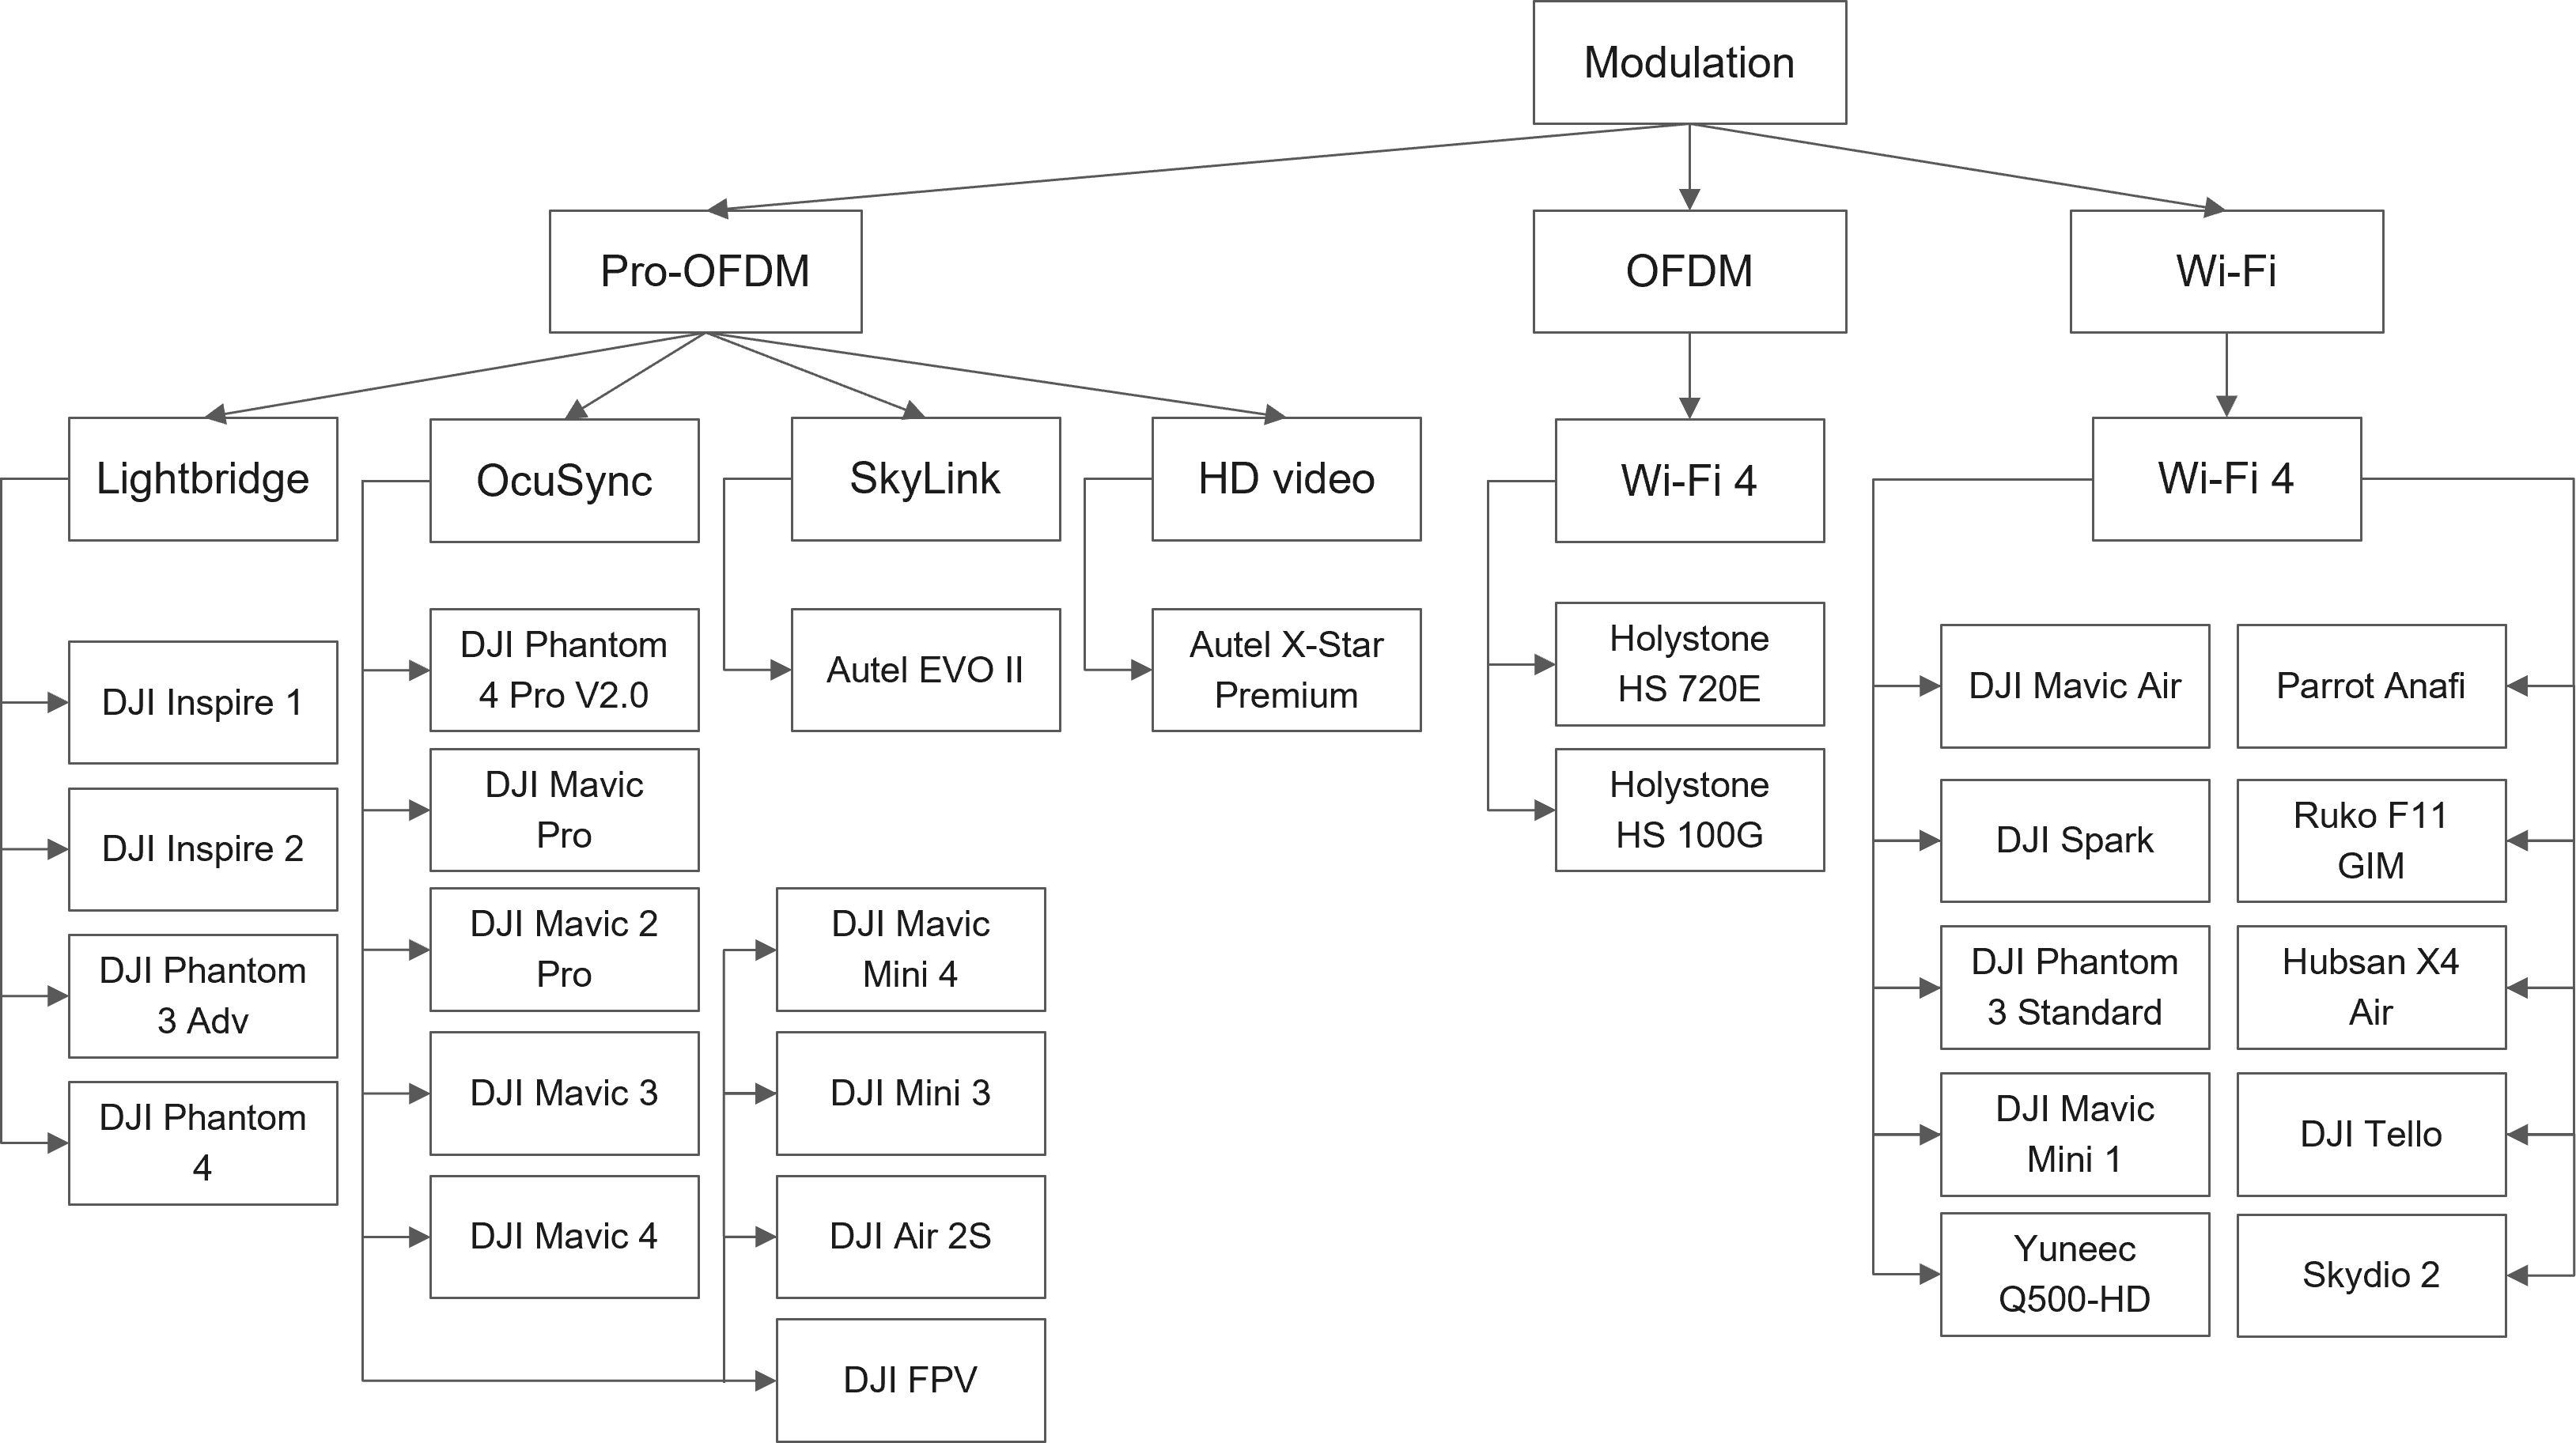
\includegraphics[width=1\linewidth]{FIGURES/cdrf/hier.png}
    \caption{Hierarchical classification tree structure of CageDroneRF.}
    \label{fig:hier}
\end{figure*}

\subsubsection{Baseline Model Architecture and Training}
We implemented a multi-task learning model using a shared ResNet-18 \cite{he2016deep} backbone to extract features from the input spectrograms. The output of the feature extractor is fed into three separate classification heads, each dedicated to one level of the hierarchy. The model is trained end-to-end using a ``HierarchicalLoss", which is a weighted sum of the cross-entropy losses from each head. 

To observe the effectiveness of our indoor data and how it generalizes to outdoor scenarios, we trained our hierarchical classifier on the indoor subset of CDRF and evaluated it on the outdoor subset. Furthermore, we examined how including outdoor data in the training set affects performance by training another model on the combined indoor and outdoor data. In both cases, the amount of indoor training data was kept constant to ensure a fair comparison. The models face challenging scenarios, including varying SNR levels, signal bandwidths, outdoor drones flying at different altitudes, distances, and the presence of various interferers.

\subsubsection{Experimental Results and Baseline Performance}

The results, shown in Fig.~\ref{fig:hier_plot}, compare the generalization performance of two training configurations when tested on outdoor data across three classification levels: Modulation, Protocol, and Model.

When the model is trained on indoor data only, it achieves moderate accuracy on lower-level features (Modulation: 69.95\%, Protocol: 66.11\%) but struggles significantly with identifying the specific drone model (42.07\%). This indicates poor domain generalization, as the model fails to adapt from indoor to outdoor environments.

In contrast, training on a combined set of indoor and outdoor data yields substantial improvements across all hierarchical levels. Accuracy increases to 89.42\% for Modulation, 87.34\% for Protocol, and 69.63\% for Model. The most significant gain of +27.56\% is observed in model-level classification, the task most sensitive to environmental shifts. This demonstrates that training on diverse, mixed-domain data is crucial for learning robust, invariant features.

\begin{figure}[phtb] 
    \centering
    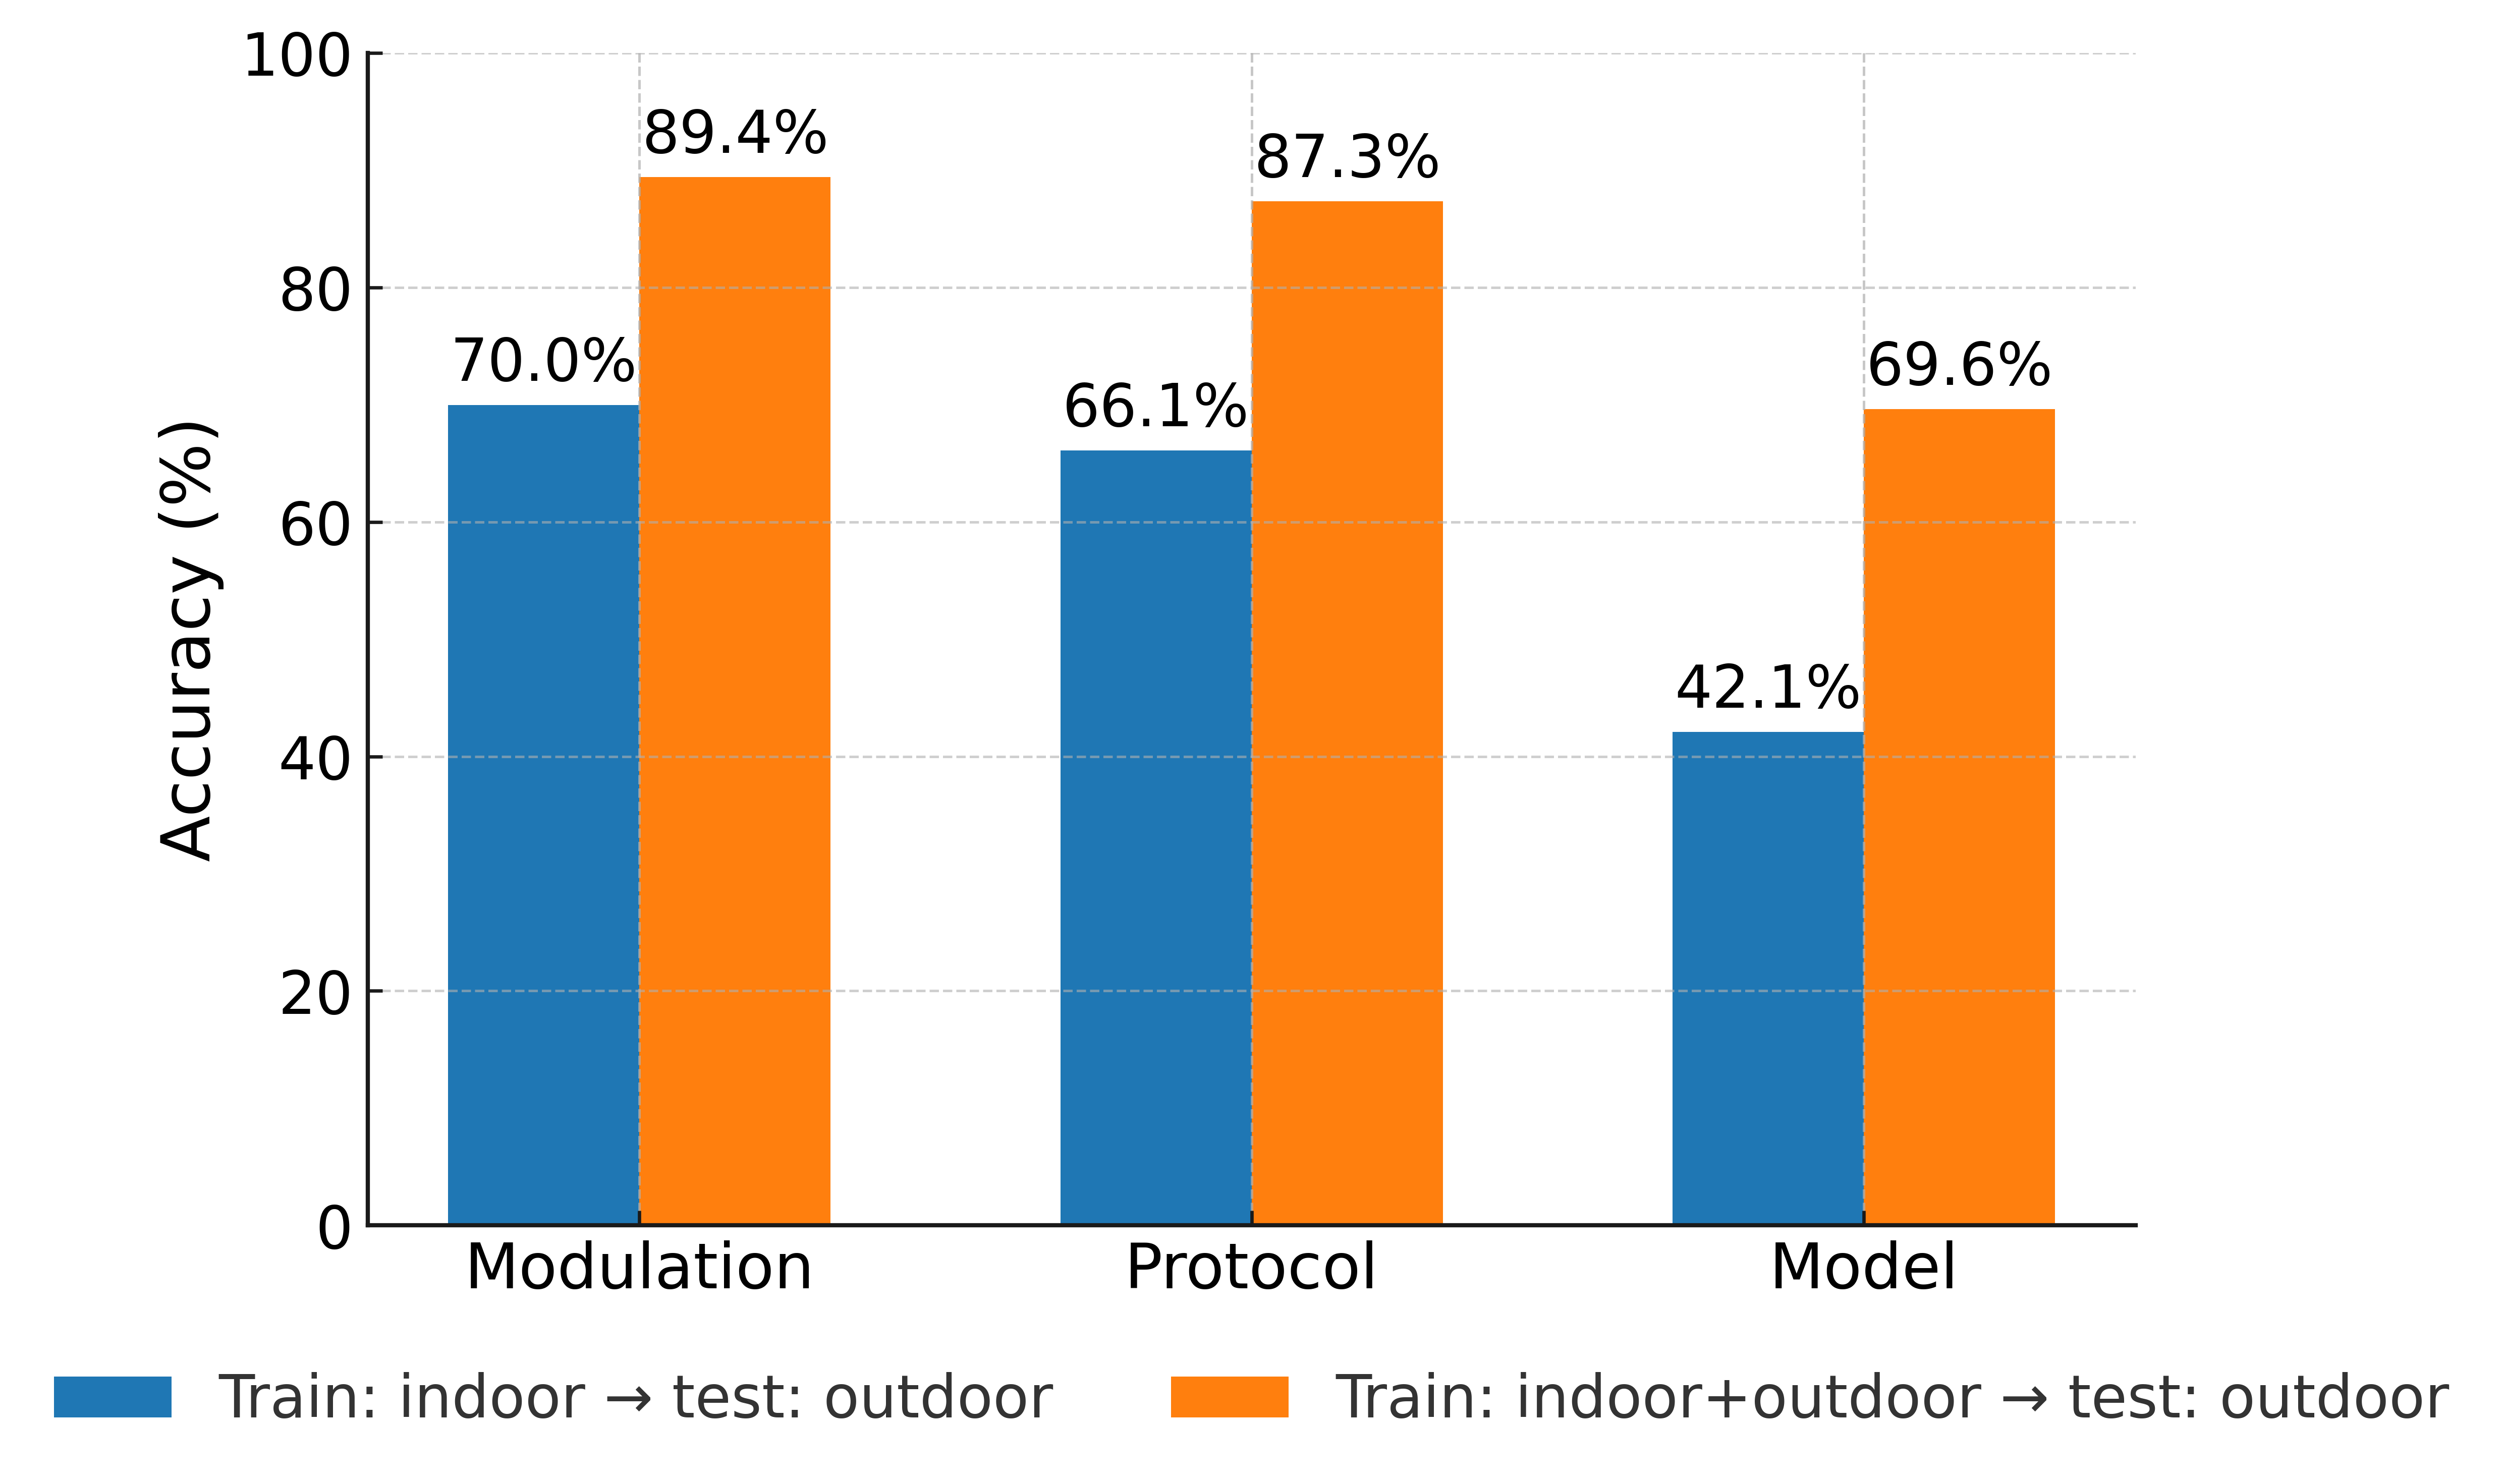
\includegraphics[width=0.7\linewidth]{FIGURES/cdrf/hier_plot.png}
    \caption{Hierarchical classification accuracy on different training setups.}
    \label{fig:hier_plot}
\end{figure}

\subsection{Open-Set Recognition}
\subsubsection{Task Definition}
Open-Set Recognition (OSR) extends classification to simultaneously: (1) accurately classify known drone types from the training set, and (2) identify and reject unknown samples as ``novel" or ``outlier" classes, preventing forced misclassification into known categories.

\subsubsection{Baseline Model Architecture and Training}
In our experiments, we utilized MetaMax \cite{lyu2023metamax}, a state-of-the-art OSR method that combines deep feature learning with statistical modeling of known class distributions. For our OSR experiments, we curated a subset of CDRF comprising 14 distinct drone types totaling 2,180 spectrogram images. The dataset was strategically partitioned into known and unknown classes to simulate realistic deployment scenarios. The known class set contains 10 drone types with 1,915 images, and the unknown class set comprises 4 drone types with 265 images. The data was split into training (60\%) and validation (20\%) samples from known classes only, with the remaining samples reserved for testing.

\subsubsection{Evaluation Metrics}
Performance metrics included: (1) closed-set accuracy on known classes, (2) unknown detection rate, and (3) overall accuracy.

\subsubsection{Experimental Results and Baseline Performance}
We evaluated MetaMax on our curated CDRF subset, achieving an overall accuracy of 75.15\%, with known class accuracy of 75.98\% and an unknown detection rate of 73.96\%. The detailed confusion matrix (Fig.~\ref{fig:osr_detailed_confusion}) reveals strong performance correlation with class size. Among the 265 unknown test samples, 196 (73.96\%) were correctly identified as novel. The binary confusion matrix for known vs. unknown discrimination is shown in Fig.~\ref{fig:osr_binary_confusion}. These results demonstrate both the promise and challenges of OSR for RF drone detection.

\begin{figure}[!ht]
    \centering
    \begin{subfigure}[h]{0.48\columnwidth}
        \centering
        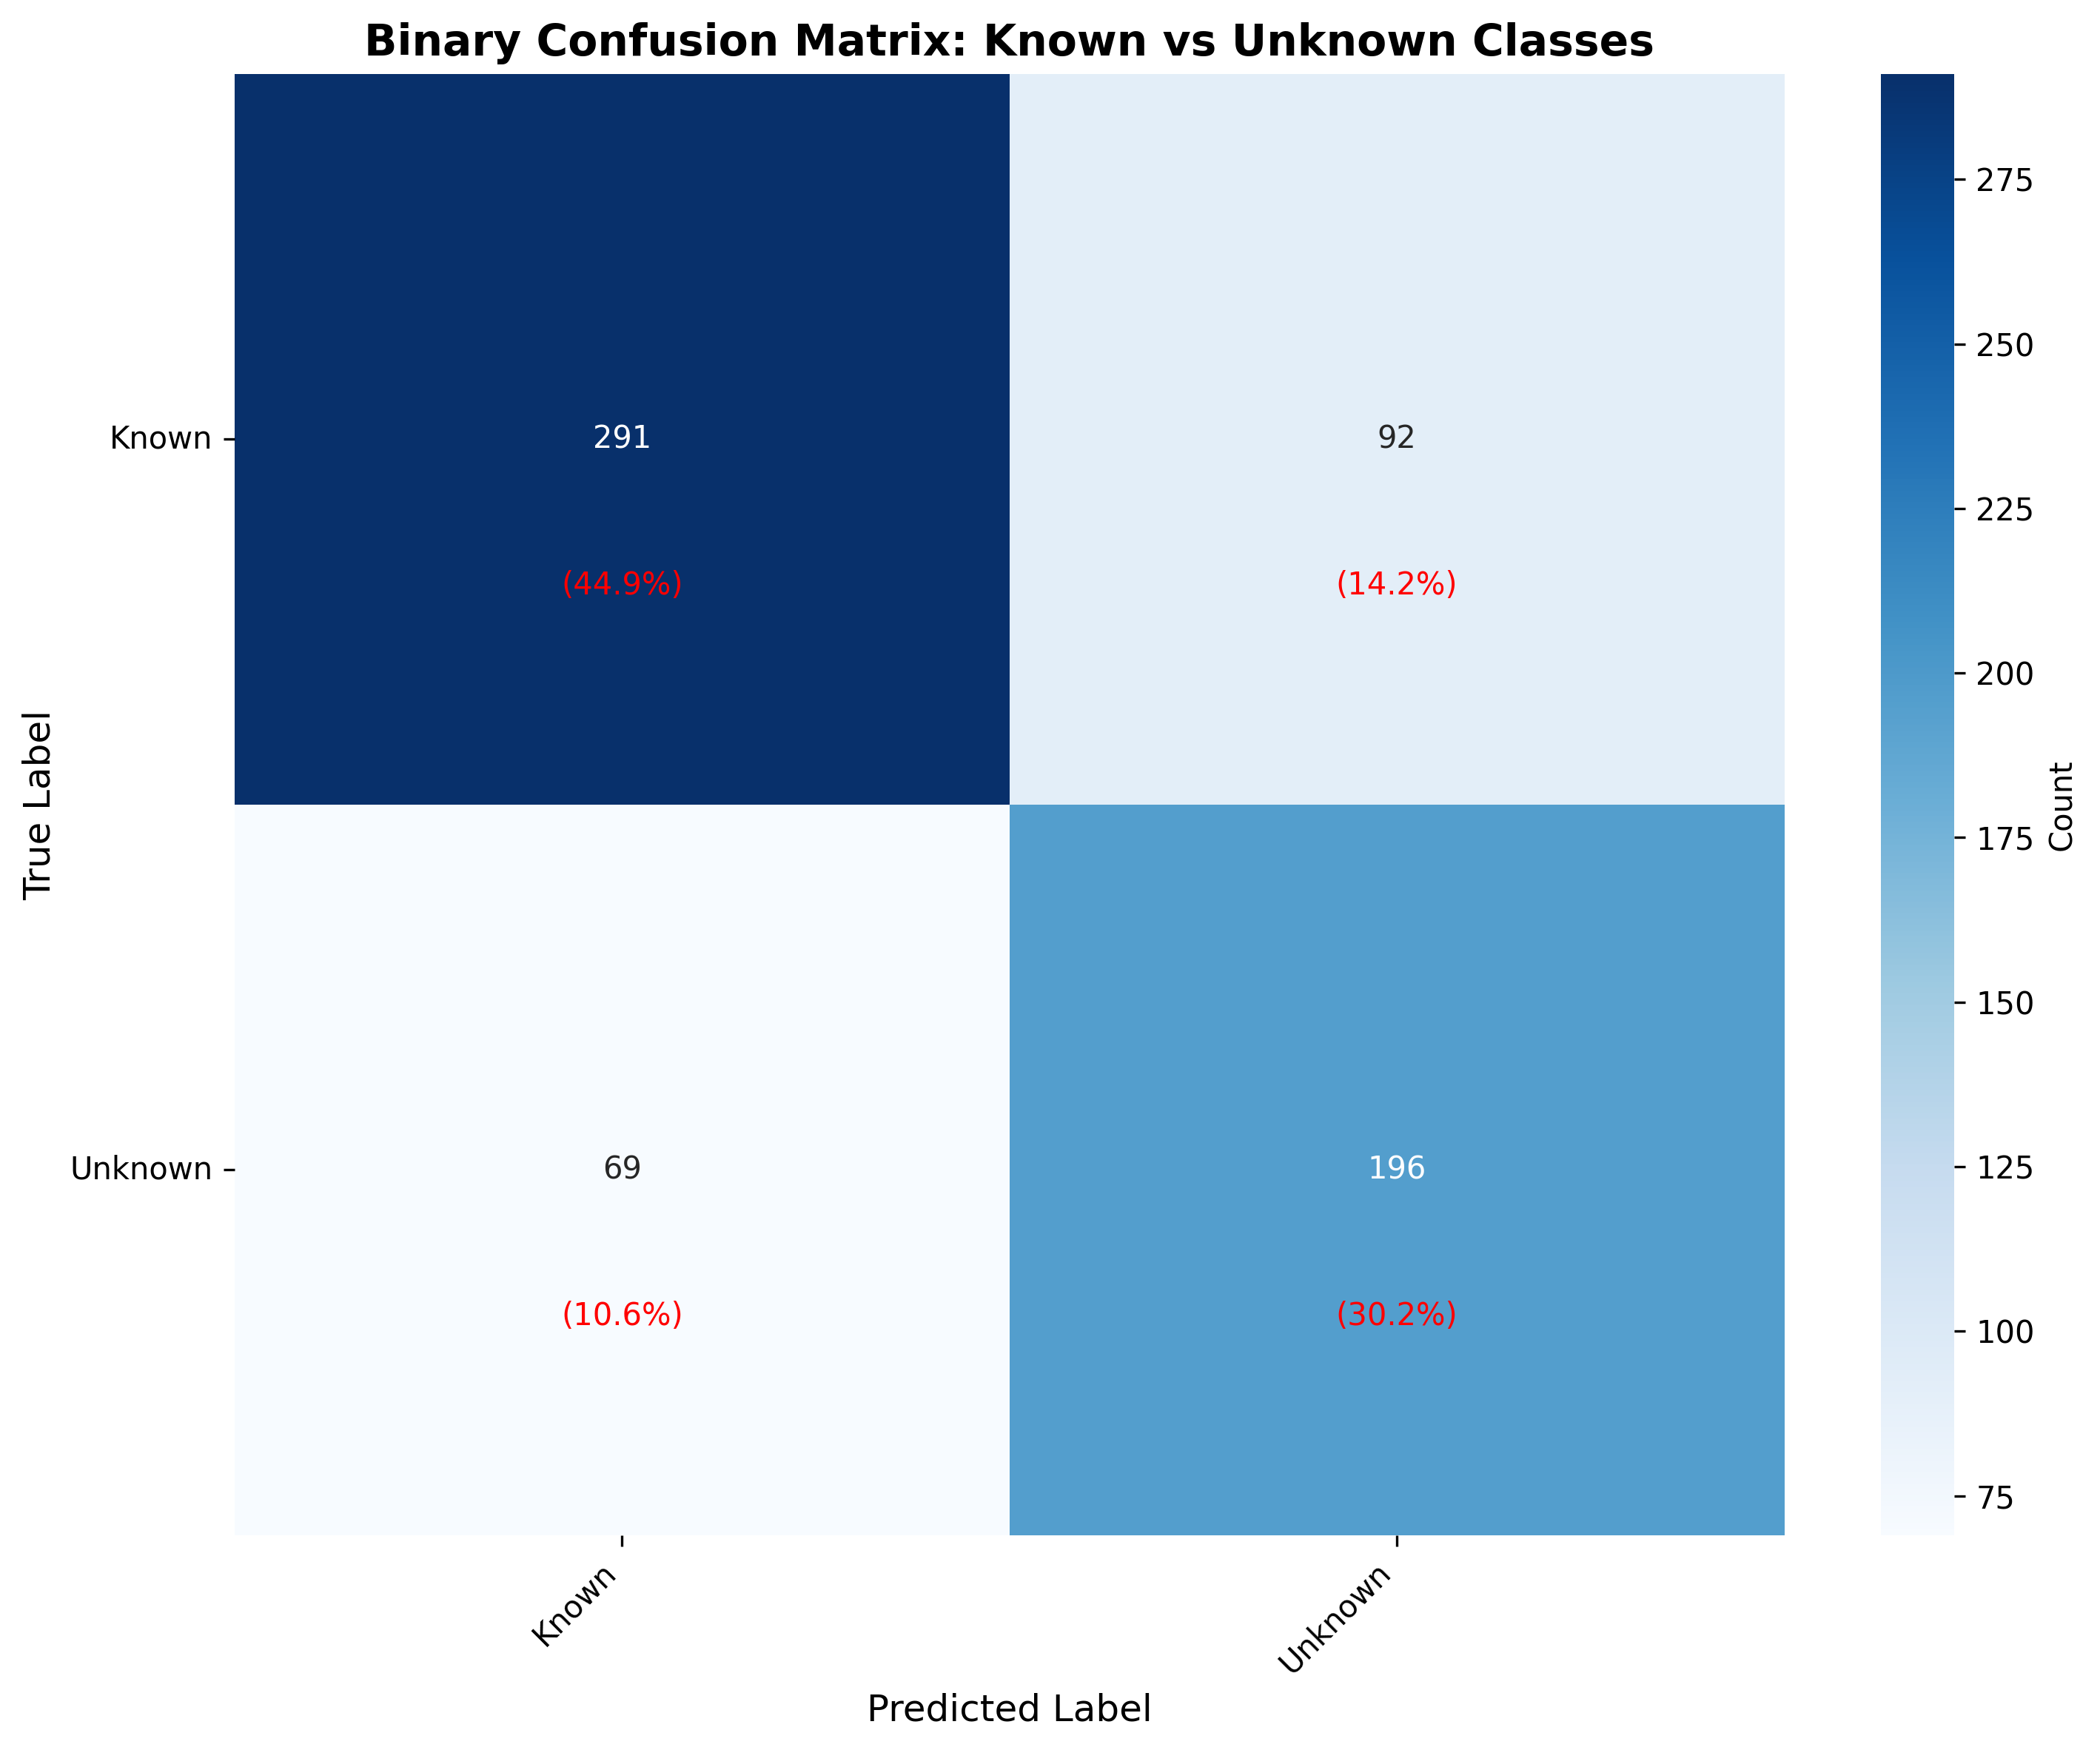
\includegraphics[width=\columnwidth]{FIGURES/cdrf/osr1.png}
        \caption{Binary confusion matrix for known vs unknown class discrimination.}
        \label{fig:osr_binary_confusion}
    \end{subfigure}
    \hfill
    \begin{subfigure}[h]{0.48\columnwidth}
        \centering
        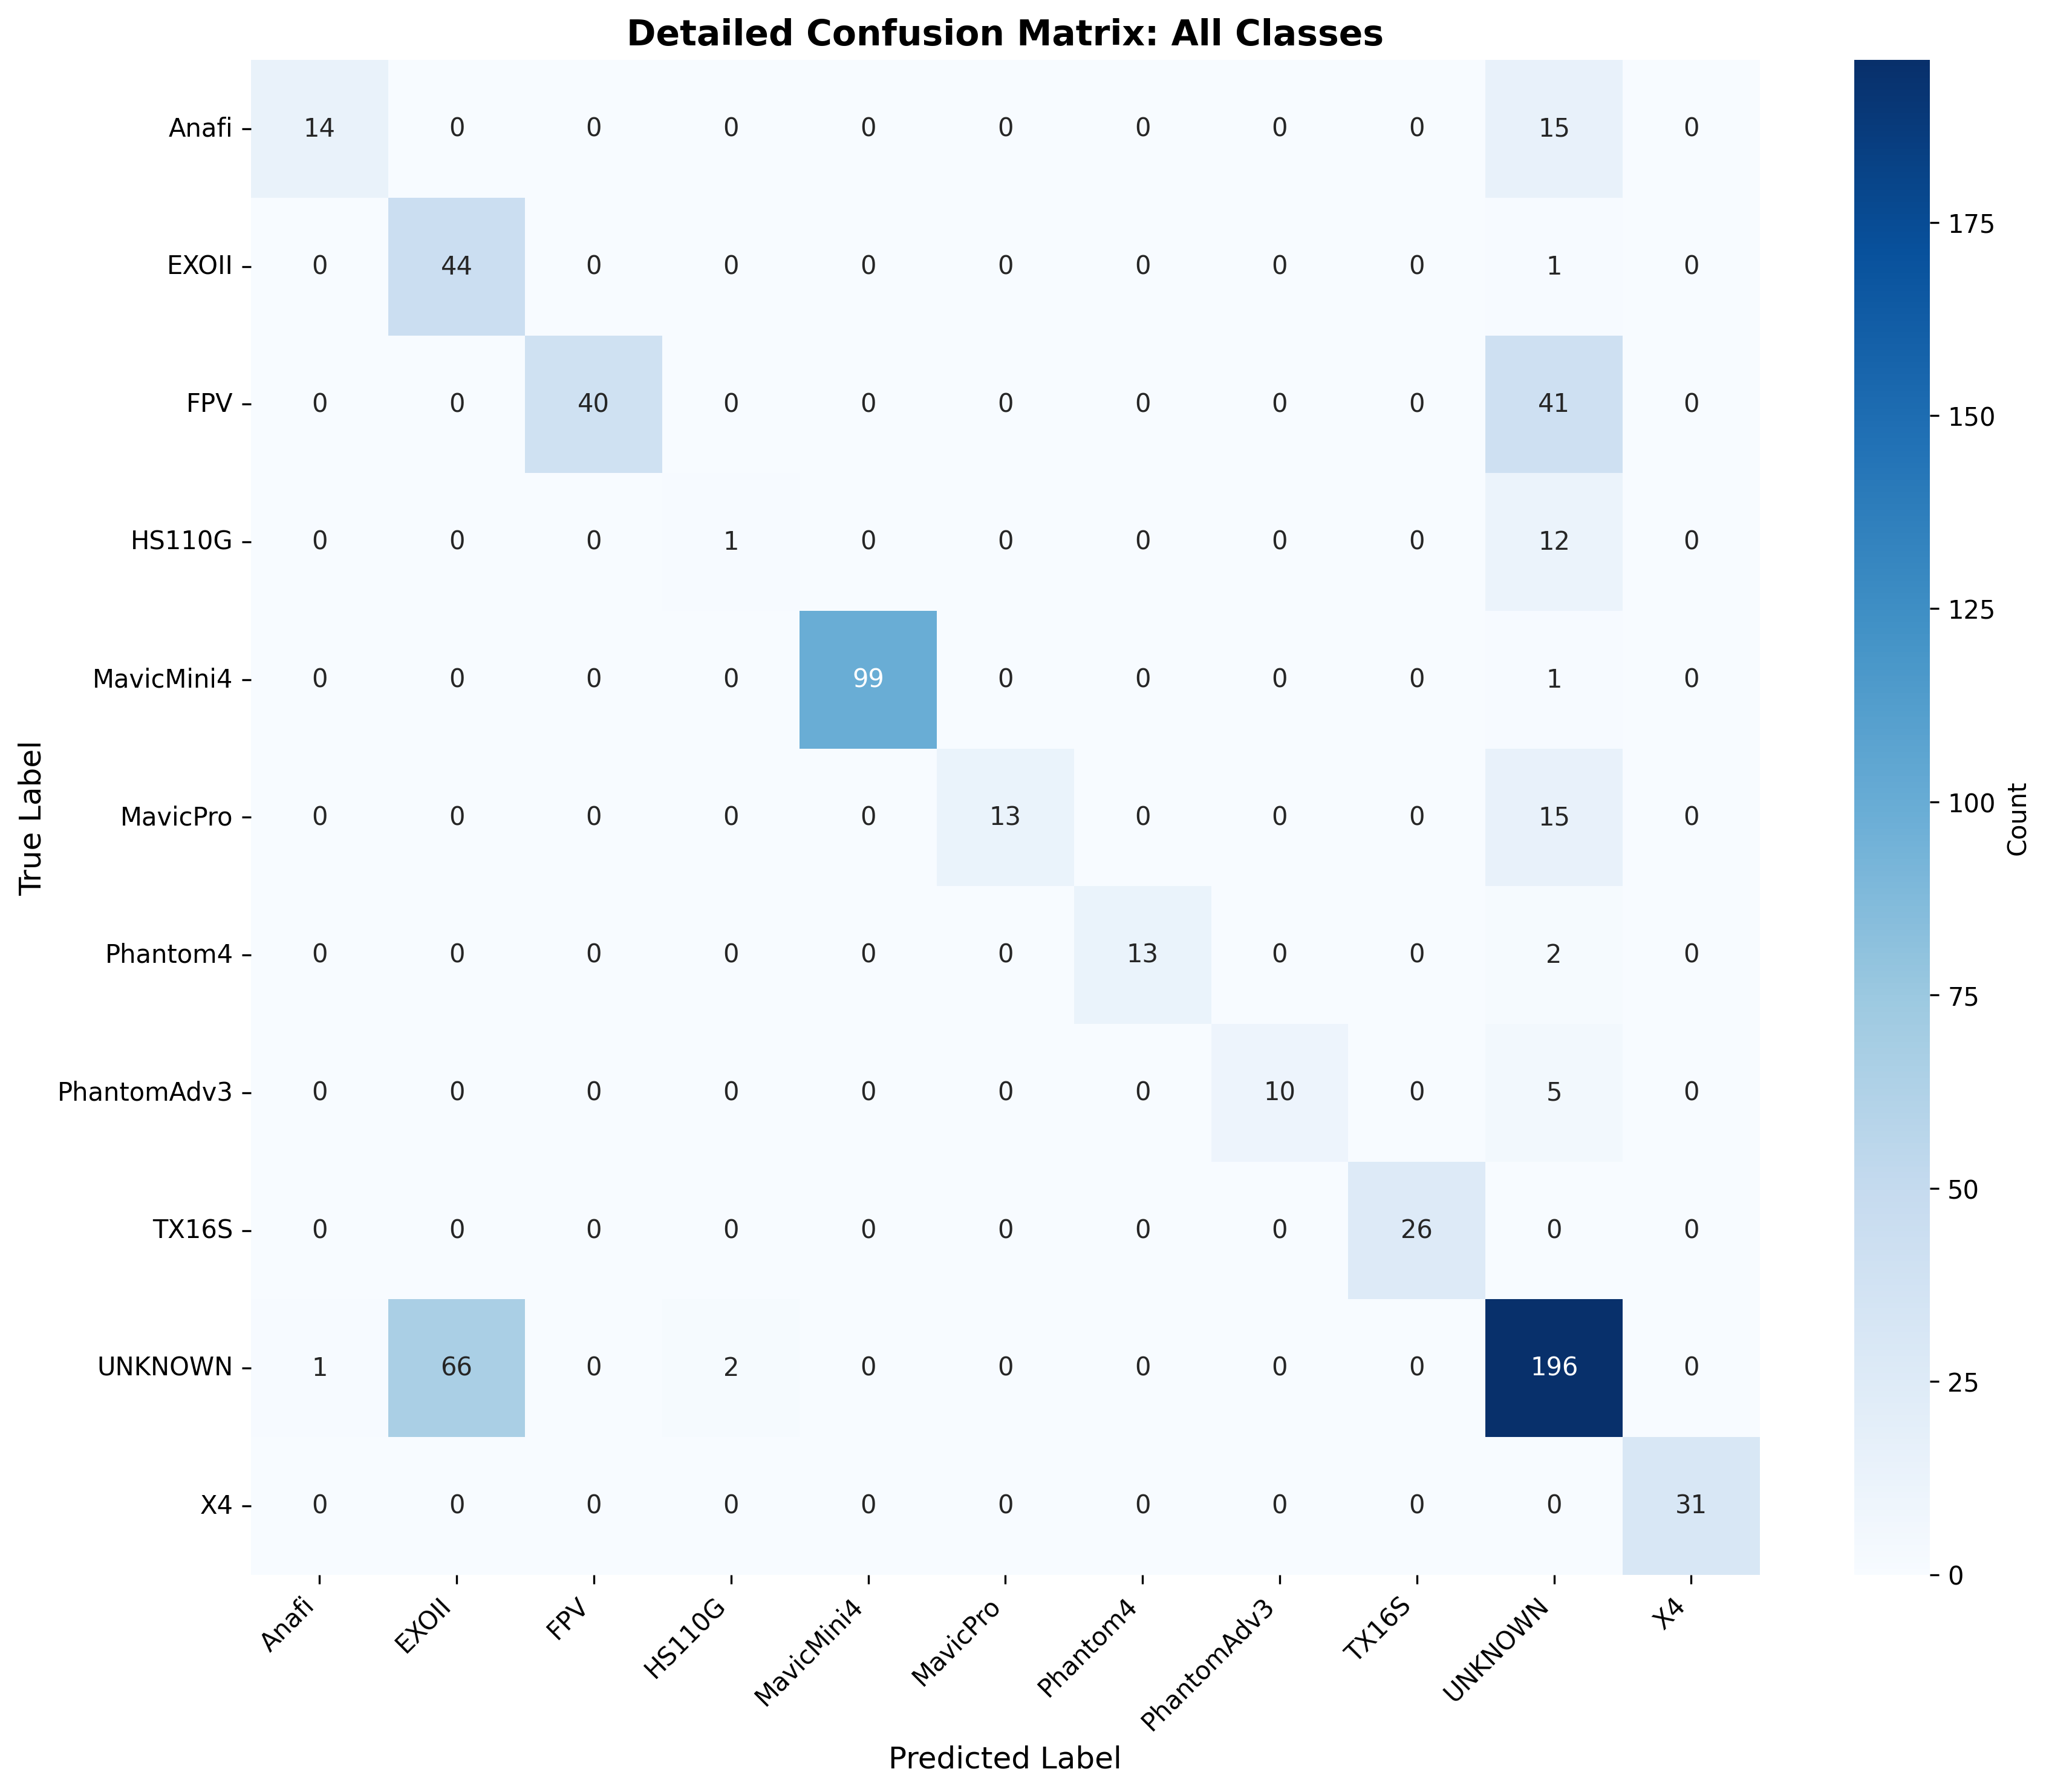
\includegraphics[width=\columnwidth]{FIGURES/cdrf/osr2.png}
        \caption{Detailed confusion matrix showing per-class performance for open-set recognition.}
        \label{fig:osr_detailed_confusion}
    \end{subfigure}
    \caption{Open-set recognition confusion matrices: (a) known vs unknown discrimination; (b) per-class detailed performance.}
    \label{fig:osr_confusions}
\end{figure}
 

\subsection{Drone Classification (Single-Label)}
\subsubsection{Task Definition}
The single-label drone classification task involves assigning each detected RF signal to exactly one drone type from a predefined set of classes.

\subsubsection{Baseline Model Architecture and Training}
We implemented a ResNet-18 convolutional neural network as the backbone, leveraging its proven effectiveness for spectrogram-based RF signal classification. The model was trained on spectrogram images generated from the CDRF dataset, using standard data augmentation and normalization techniques to improve generalization. We had a total number of 20 different drone types in our dataset. The ResNet-18 model was trained with a cross-entropy loss and optimized using Adam.
 
\subsubsection{Experimental Results and Baseline Performance}

After training, the model achieved a test accuracy of 53.49\%, as shown in the confusion matrix (Fig.~\ref{fig:flat_confusion_matrix}). The confusion matrix reveals that certain drone types are classified with high accuracy, while others exhibit significant misclassifications, especially for classes that seen less training data, indicating areas for potential improvement. The results highlight the challenges of single-label classification in RF drone signals, particularly in distinguishing between similar models.

\begin{figure}[!ht]
    \centering
    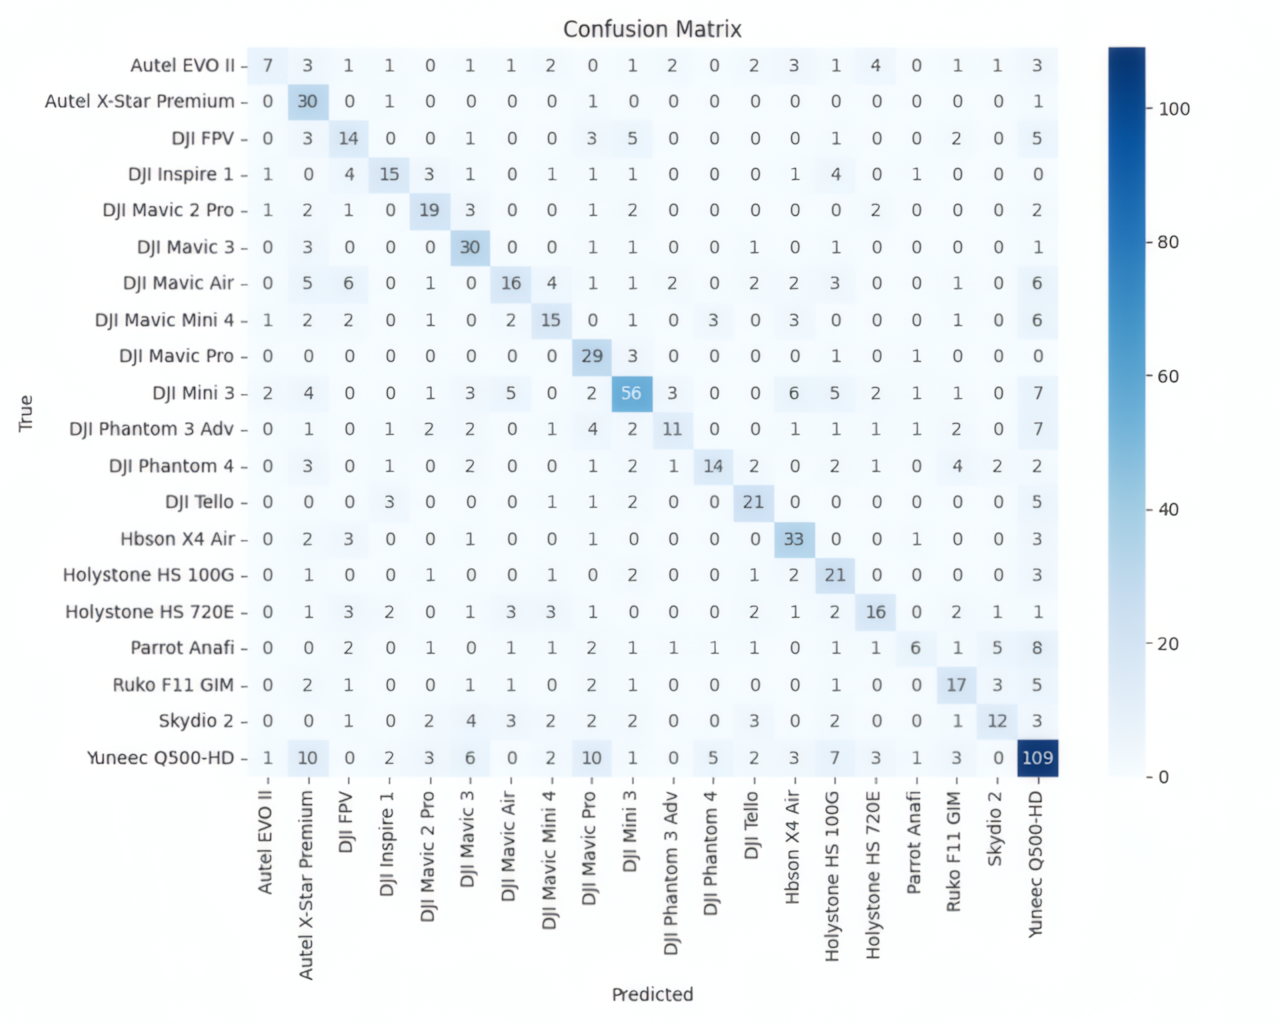
\includegraphics[width=\columnwidth]{FIGURES/cdrf/label.png}
    \caption{Confusion matrix for single-label drone classification.}
    \label{fig:flat_confusion_matrix}
\end{figure}

% TODO: Omiting Multi-Label results for conciseness.
% \subsection{Multi-Label Classification}
% \subsubsection{Task Definition}
% This work addresses the specific problem of identifying multiple drone models in a single image, a task known as multi-label classification.

% \subsubsection{Baseline Model Architecture and Training}
% To adapt a standard classification model for this task, a key architectural change is required in the final output layer. We replace the softmax activation function with the sigmoid activation function applied independently to each output neuron. Consequently, the loss function is changed from Categorical Cross-Entropy to Binary Cross-Entropy. We use a ResNet18 backbone for handling the multi-label classification task.

% The dataset is prepared by creating multi-hot encoded labels for each image, where each label vector indicates the presence (1) or absence (0) of each drone model. In our experiment, we used 3 different drone classes: DJI FPV, DJI Mavic3, DJI Mini3. In each dataset two drones were presented and this combination provided 3 different classes of multilabel data. The model was trained using the Adam optimizer with a learning rate of 0.001 and a batch size of 32 for 5 epochs.

% \subsubsection{Evaluation Metrics}
% The performance was evaluated using per-class precision, recall, and F1-score, as well as overall accuracy.

% \subsubsection{Experimental Results and Baseline Performance}
% The model obtained a perfect overall accuracy of 100\%, with precision, recall, and F1-score of 100\% for each class. The results demonstrated the model's ability to effectively identify multiple drone models within a single image.


\section{Discussion and Future Work}
\label{sec:discussion}

\textbf{Cross-Modal Transfer Validation:} CDRF's results validate the central hypothesis underlying the dissertation's framework: vision models successfully transfer to wireless domains when signals are represented as images. The YOLOv11n detector achieves mAP@0.5 = 0.986 on clean spectrograms and 0.935 under augmentation, demonstrating that object detection architectures pretrained on natural images (COCO) extract meaningful features from RF time-frequency representations without wireless-specific modifications. Similarly, ResNet-18 baselines achieve 53.49\% single-label accuracy across 20 drone types and 75.98\% known-class accuracy in open-set scenarios, confirming that convolutional architectures transfer across modalities. This empirical evidence directly supports Research Question 1 (RQ1) and justifies DenoMAE's approach of leveraging vision transformers for wireless representation learning (Chapter~\ref{chap:denomae}).

\textbf{Robustness Gap and Foundation Model Implications:} The performance degradation under augmented conditions reveals critical challenges for foundation models. The recall drop from 0.982 to 0.855 (YOLOv11n) reflects the precision-recall tradeoff when training on low-SNR, high-interference conditions: the detector becomes more conservative to avoid false positives but misses more true detections. This robustness gap motivates the dissertation's modular framework: self-supervised pretraining (DenoMAE) on diverse unlabeled signals should learn noise-invariant representations; LLM-based reasoning (Plug-and-Play) should provide complementary decision-making that doesn't degrade under noise; and meta-learning (Meta-Task) should enable rapid adaptation to deployment-specific SNR distributions with minimal labeled data. The hierarchical classification results (indoor-only: 42.07\% model accuracy; mixed training: 69.63\%, +27.56\%) demonstrate that domain shift, a core challenge for foundation models, can be addressed through diverse pretraining data, validating the framework's emphasis on broad data coverage.

\textbf{Open-Set Recognition and Real-World Deployment:} The 73.96\% unknown detection rate establishes that models can learn to reject novel threats, but the class-size correlation in performance (Fig.~\ref{fig:osr_detailed_confusion}) highlights a persistent challenge: data imbalance. This finding connects directly to Meta-Task (Chapter~\ref{chap:meta_task}), which addresses few-shot learning scenarios where new drone types emerge with only 5-10 labeled examples. The open-set capability validated here provides a safety mechanism for foundation model deployment: rather than forcing every input into a known category, models can flag uncertainty and request human verification.

\textbf{Confounded Comparisons and Split Provenance:} Two methodological caveats bound the results above. First, the indoor-only versus indoor+outdoor hierarchical comparison (42.07\% vs.\ 69.63\% model-level accuracy) changes both domain coverage and training population size simultaneously, since the indoor-only condition was not also evaluated with a matched, enlarged indoor-only sample; the reported gain should therefore be attributed to the combination of more data and more diverse data, not cleanly isolated to domain diversity alone. Second, this chapter does not ship a recording/session/device-level split manifest proving that augmented or time-windowed descendants of the same raw recording never cross a train/validation/test boundary. Repeated windows or synthetic descendants from one raw recording are statistically related, so a large number of generated images is not automatically a large number of independent acquisition conditions; without a published lineage manifest, the independence of the reported splits cannot currently be audited externally. This is an absence of documented evidence rather than a demonstrated leakage finding, and releasing such a manifest is a priority for future releases of CDRF.

To ensure the long-term relevance and utility of CDRF, we are committed to its continuous expansion. Future work will focus on several key areas:
% \todo[inline,color=blue!40]{To Everyone: Do we want to make this commitment?}
\begin{itemize}
    \item \textbf{Dataset Expansion:} We will regularly update the dataset with new and emerging drone models, as well as more diverse background and interference signals captured from a wider range of environments (e.g., urban, industrial, and rural). We also plan to integrate CDRF with other public datasets to create an even more comprehensive and diverse benchmark.
    \item \textbf{Advanced Model Architectures:} We will explore the application of more sophisticated deep learning models, such as Transformers and graph neural networks, which may be better suited to capturing the complex temporal and spectral dependencies in RF signals.
    \item \textbf{Enhanced Augmentation Techniques:} We will continue to develop more advanced data augmentation techniques that can more realistically simulate a wider range of real-world channel effects, such as multipath fading and Doppler shifts.
    \item \textbf{Focus on Advanced Tasks:} We will further investigate the more challenging tasks of multi-label and open-set classification, which are critical for real-world applications where multiple drones may be present, and novel threats are a constant concern.
\end{itemize}

\section{Conclusion}
\label{sec:crdf_conclusion}

This chapter presented CDRF, a comprehensive benchmark that validates a fundamental premise of the dissertation's framework: vision models can successfully transfer to wireless perception tasks. By demonstrating that YOLO detection (mAP@0.5 = 0.986 clean, 0.935 augmented) and ResNet classification operate effectively on RF spectrograms, CDRF provides empirical evidence for the cross-modal transfer principle underlying Research Question 1 (RQ1). This validation justifies the multimodal approach pursued in DenoMAE (Chapter~\ref{chap:denomae}), where masked autoencoders learn universal wireless representations by treating signals as images.

Beyond theoretical validation, CDRF establishes a realistic stress-test benchmark for foundation model components. The performance degradation under augmented conditions, particularly the recall drop from 0.982 to 0.855 in YOLO detection, reveals the robustness challenges that operational systems face. The hierarchical classification results (+27.56\% model-level gain with mixed indoor/outdoor training) demonstrate the domain shift problem that foundation models must address through diverse pretraining and effective adaptation mechanisms. The open-set recognition capability (73.96\% unknown detection) validates that models can learn to reject novel threats, a critical requirement for real-world deployment.

\textbf{Framework Integration:} Within the dissertation's modular system, CDRF serves three essential roles. First, it validates the feasibility of vision-to-wireless transfer, establishing that pre-trained computer vision architectures provide a strong foundation for wireless perception. Second, it provides a diverse, challenging benchmark (39 classes, 500GB raw data, controlled SNR stratification) for evaluating whether foundation model approaches, namely self-supervised learning (DenoMAE), LLM-based reasoning (Plug-and-Play), and meta-learning adaptation (Meta-Task), generalize beyond clean laboratory conditions. Third, its raw-signal augmentation pipeline and dataset-agnostic tooling enable systematic robustness evaluation across the SNR, interference, and domain shift conditions that real deployments encounter.

The success of vision models on CDRF's drone detection tasks demonstrates that cross-modal knowledge transfer is not merely theoretical but practically achievable. This empirical validation provides confidence for pursuing the more sophisticated approaches in subsequent chapters: DenoMAE's self-supervised representation learning can leverage vision transformer architectures because those architectures demonstrably work for wireless signals; the Plug-and-Play framework's LLM integration becomes more plausible given that one domain (vision) has already successfully transferred to wireless; and Meta-Task's few-shot adaptation addresses the remaining challenge of rapidly specializing foundation model capabilities to new wireless scenarios with minimal data.

By open-sourcing both dataset and toolkit, CDRF aims to foster reproducible research and collaborative progress toward robust, field-ready wireless AI systems. Future work will expand the dataset with emerging drone models, explore advanced architectures (transformers, graph neural networks), and investigate how CDRF can serve as a pretraining corpus or evaluation benchmark for the integrated foundation model framework proposed in this dissertation.
    


